\documentclass[12pt]{article}
\usepackage[backend=bibtex]{biblatex}
\addbibresource{references.bib}
\usepackage{hyperref}
\usepackage[utf8]{inputenc}
\usepackage[brazil]{babel}
\usepackage[lmargin=3cm,tmargin=3cm,rmargin=2cm,bmargin=2cm]{geometry}
\usepackage[T1]{fontenc}
\usepackage{lmodern}
\usepackage{setspace}
\usepackage{amsmath, amsfonts, amsthm, amssymb, dsfont, mathtools}
\usepackage{graphicx}
\usepackage{subfig}
\usepackage{indentfirst}
\usepackage{fancyhdr}
\lhead{ }
\chead{ }
\rhead{ }
\lfoot{ }
\cfoot{ }
\rfoot{\thepage}
\renewcommand{\headrulewidth}{0pt}

\title{\textbf{Análise de Transcriptogramas na Transição Epitélio-Mesenquimal (EMT)}}
\author{Odilon Júlio dos Santos}
\date{2025}

\begin{document}

%%%%%% CAPA %%%%%%
\begin{center}
\begin{figure}
    \centering
    
\includegraphics[width=0.25\linewidth]{brasao_gradiente.png}
\end{figure}
\textbf{UNIVERSIDADE FEDERAL DO RIO GRANDE DO NORTE}

\textbf{PROGRAMA DE PÓS-GRADUAÇÃO EM BIOINFORMÁTICA}

\vfill

\textbf{Análise de Transcriptogramas na Transição Epitelio-Mesenquimal (EMT)}

\vfill

\textbf{Odilon Júlio dos Santos}

\vfill

Dissertação apresentada ao Programa de Pós-Graduação em Bioinformática da Universidade Federal do Rio Grande do Norte, como requisito parcial para a obtenção do título de Mestre em Bioinformática.

\vfill

Orientadora: Prof\textsuperscript{a}. Dra. Rita Maria Cunha de Almeida\\
Coorientador: Prof\textsuperscript{o}. Dr. Rodrigo Juliani Siqueira Dalmolin

\vfill

Natal - RN\
2025

\end{center}

\newpage

%%%%%% RESUMO %%%%%%
\begin{center}
\textbf{RESUMO}
\end{center}

A Transição Epitélio-Mesenquimal (EMT) é um processo biológico essencial para o desenvolvimento embrionário, cicatrização tecidual e progressão tumoral. Este estudo investiga as alterações transcricionais durante a EMT utilizando dados de Single-Cell RNA-seq de células MCF10A tratadas com TGF-$\beta$1 em diferentes períodos. Os dados foram retirados do estudo publicado na PNAS (2021) (DOI: 10.1073/pnas.2102050118).
Os dados foram coletados em dois batchs experimentais para capturar variações temporais: Batch 1: Dias 0, 4 e 8 de tratamento. Batch 2: Dias 0, 1, 2 e 3 de tratamento. A presença de dois batchs exigiu correção de efeitos de batch, feita pela normalização das expressões gênicas entre os dias zero de ambos os lotes. A normalização envolveu a divisão dos valores pelo total de leituras da célula, seguida pela aplicação da razão entre as médias dos controles.
A análise foi realizada utilizando o pacote Transcriptogramer, que projeta perfis de expressão gênica em uma lista ordenada de proteínas baseada em interações proteína-proteína. O método permite a identificação de padrões transcricionais contínuos e o agrupamento de genes co-expressos. A Análise de Componentes Principais (PCA) foi utilizada para visualizar variações na expressão gênica ao longo da EMT, sem escalonamento (scale=FALSE), preservando a variação biológica original.
Foram gerados transcriptogramas para representar a dinâmica da EMT, identificando genes diferencialmente expressos e possíveis estágios parciais do processo. Os resultados obtidos até o momento sugerem padrões distintos de expressão gênica entre os batchs, reforçando a importância da correção de batch effects. A reconstrução dos transcriptogramas revelou agrupamentos funcionais, destacando genes chave na EMT.
Entre as próximas etapas, estão a reconstrução dos transcriptogramas para algumas amostras, a seleção dos genes mais variáveis ao longo do tempo e a clusterização por co-expressão, visando definir uma lista de genes que melhor descrevem a EMT nesse contexto. Além disso, buscamos obter uma descrição detalhada da evolução da expressão gênica ao longo da EMT que possa servir como base para modelos computacionais de órgãos e tecidos virtuais, permitindo futuras aplicações em simulações biomédicas.


\textbf{Palavras-chave:} Transição Epitélio-Mesenquimal (EMT); Single-Cell RNA-seq;
Células MCF10A;
Tratamento com TGF-$\beta$ 1;
Correção de efeito de batch;
Normalização da expressão gênica;
Análise de transcriptograma;
Interações proteína-proteína;
Análise de Componentes Principais (PCA);
Expressão gênica diferencial;
Clusterização por co-expressão;
Padrões temporais de expressão gênica;


\newpage

%%%%%% ABSTRACT %%%%%%
\begin{center}
\textbf{ABSTRACT}
\end{center}

Epithelial-Mesenchymal Transition (EMT) is a biological process essential for embryonic development, tissue healing, and tumor progression. This study investigates transcriptional changes during EMT using Single-Cell RNA-seq data from MCF10A cells treated with TGF-$\beta$1 at different time points. The data were obtained from the study published in PNAS (2021) (DOI: 10.1073/pnas.2102050118). Samples were collected in two experimental batches to capture temporal variations: Batch 1: Days 0, 4, and 8 of treatment. Batch 2: Days 0, 1, 2, and 3 of treatment. The presence of two batches required batch effect correction, which was performed by normalizing gene expression between the day 0 samples from both batches. The normalization involved dividing expression values by the total number of reads per cell, followed by applying the ratio of the mean expression values of the control samples. The analysis was conducted using the Transcriptogramer package, which projects gene expression profiles onto an ordered list of proteins based on protein-protein interactions. This method enables the identification of continuous transcriptional patterns and the clustering of co-expressed genes. Principal Component Analysis (PCA) was employed to visualize gene expression variations throughout EMT without scaling (scale=FALSE), preserving the original biological variation. Transcriptograms were generated to represent EMT dynamics, identifying differentially expressed genes and potential partial stages of the process. The results obtained so far suggest distinct gene expression patterns between batches, reinforcing the importance of batch effect correction. The reconstruction of transcriptograms revealed functional clusters, highlighting key genes involved in EMT. Future steps include reconstructing transcriptograms for selected samples, identifying the most variable genes over time, and clustering genes based on co-expression to define a list of genes that best describe EMT in this context.

\textbf{Keywords:} Epithelial-Mesenchymal Transition (EMT); Single-Cell RNA-seq; MCF10A cells; TGF-$\beta$1 treatment; Batch effect correction; Gene expression normalization; Transcriptogram analysis; Protein-protein interactions; Principal Component Analysis (PCA); Differential gene expression; Co-expression clustering; Temporal gene expression patterns.

\newpage

\section{Introdução}

A análise da expressão gênica tem sido amplamente utilizada para compreender mecanismos biológicos complexos, permitindo a identificação de padrões diferenciais de regulação gênica e agrupamentos funcionais. No entanto, métodos convencionais frequentemente não consideram as interações funcionais entre genes, limitando a interpretação dos dados.

O método \textit{Transcriptogramer} surge como uma abordagem inovadora para integrar informações de expressão gênica com redes de interação proteína-proteína (PPI). Ao projetar os dados em uma lista ordenada de proteínas e aplicar suavização por janelas deslizantes, esse método permite uma análise mais robusta da regulação gênica, facilitando a identificação de padrões biológicos relevantes.

Neste estudo, utilizamos o \textit{Transcriptogramer} para analisar dados de expressão gênica de \textit{single-cell RNA-Seq} (\textit{scRNA-Seq}), com foco na transição epitélio-mesenquimal (EMT), um processo fundamental em diversos contextos biológicos, incluindo desenvolvimento embrionário, cicatrização e progressão tumoral. Além disso, realizamos análises comparativas utilizando diferentes valores de raio ($r = 0$ e $r = 30$) e empregamos Análise de Componentes Principais (PCA) para avaliar a variação global dos dados e otimizar a dimensionalidade das informações.

\section{Transição Epitélio-Mesenquimal}

A \textbf{Transição Epitélio-Mesenquimal (EMT)} é um processo biológico fundamental no qual células epiteliais perdem suas características típicas, como adesão celular e polaridade, e adquirem um fenótipo mesenquimal, caracterizado por maior motilidade e capacidade de invasão. Esse fenômeno desempenha um papel essencial em vários contextos fisiológicos e patológicos, incluindo desenvolvimento embrionário, cicatrização de feridas e progressão tumoral \cite{dongre}.



A EMT é um processo biológico essencial, com profundas implicações no desenvolvimento, cicatrização e progressão do câncer. Estudos recentes baseados em \textbf{single-cell RNA sequencing} têm revelado a complexidade desse fenômeno, sugerindo que sua regulação é altamente dinâmica e influenciada por múltiplos fatores. A compreensão aprofundada da EMT pode fornecer novos alvos terapêuticos para tratar doenças associadas à plasticidade celular.

% \begin{figure}
%     \centering
%     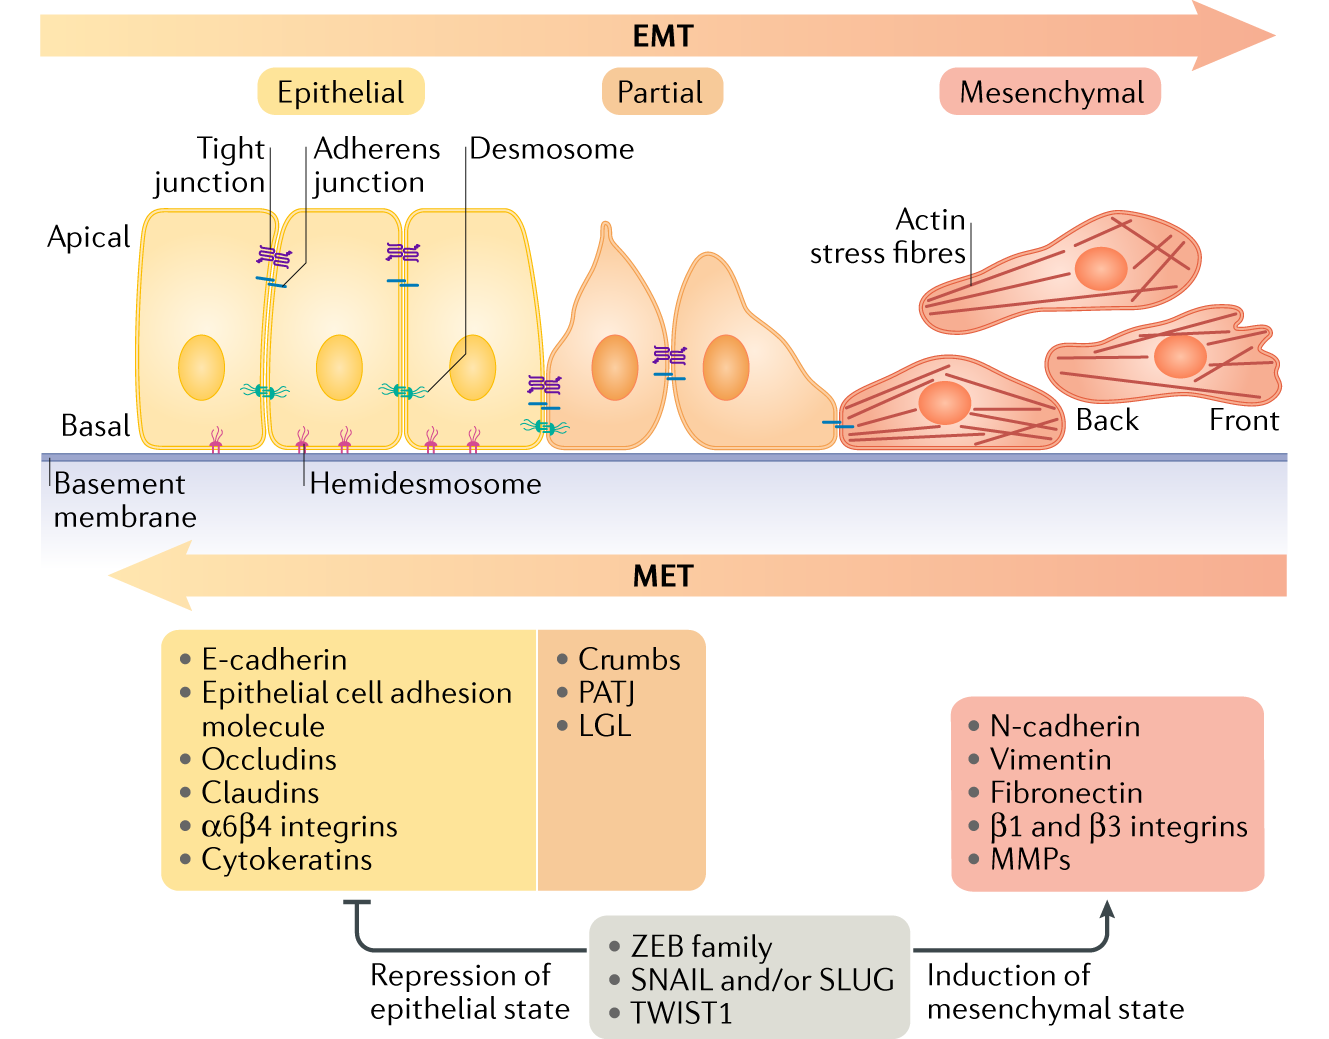
\includegraphics[width=0.75\linewidth]{EMT.png}
%     \caption{Transição Epitélio-Mesenquimal. Fonte: \href{https://doi.org/10.1073/pnas.2102050118}{Deshmukh et al., 2021}.}
%     \label{fig:enter-label}
% \end{figure}

\subsection{Aspectos Moleculares da EMT}

A EMT é regulada por uma complexa rede de fatores de transcrição, vias de sinalização e alterações epigenéticas. Entre os principais reguladores da EMT estão os fatores \textbf{SNAIL}, \textbf{TWIST} e \textbf{ZEB}, que reprimem a expressão de genes epiteliais, como \textbf{E-caderina (CDH1)}, e ativam genes associados ao fenótipo mesenquimal, como \textbf{N-caderina (CDH2)} e \textbf{vimentina (VIM)} \cite{deshmukh}. Além disso, vias de sinalização como \textbf{TGF-$\beta$}, \textbf{WNT, NOTCH} e \textbf{Hedgehog} desempenham papéis críticos na indução da EMT \cite{dongre}.

\subsection{Fases da EMT}

A EMT pode ser descrita em um espectro de estados celulares, desde um fenótipo epitelial puro até um fenótipo mesenquimal totalmente estabelecido. Estudos recentes utilizando sequenciamento de RNA de célula única indicam que a EMT não é um evento binário, mas sim um continuum de transição celular, no qual células podem apresentar estados híbridos, conhecidos como \textbf{epitélio-mesenquimais intermediários} \cite{deshmukh}. Essa plasticidade celular é de grande relevância na progressão do câncer, pois permite que células tumorais adquiram propriedades de invasão e resistência a terapias.

\subsection{EMT e Progressão Tumoral}

Na oncologia, a EMT está fortemente associada à metástase, permitindo que células epiteliais malignas adquiram a capacidade de migrar e invadir tecidos adjacentes. Durante esse processo, a EMT confere resistência a terapias convencionais, tornando o tratamento de certos tipos de câncer mais desafiador \cite{dongre}. Além disso, células que passam pela EMT podem contribuir para a formação de \textbf{células-tronco cancerígenas (CSC, do inglês Cancer Stem Cells)}, um subgrupo de células tumorais com alta capacidade de auto-renovação e resistência terapêutica \cite{deshmukh}.

\subsection{Reversibilidade da EMT e Transição Mesenquimal-Epitelial}

Curiosamente, a EMT não é um evento irreversível. Células que passaram por esse processo podem reverter para um fenótipo epitelial por meio da \textbf{Transição Mesenquimal-Epitelial (MET)}. Esse mecanismo é observado durante o estabelecimento de metástases secundárias, onde células mesenquimais migrantes colonizam um novo tecido e readquirem características epiteliais para formar uma nova massa tumoral \cite{dongre}. Compreender os mecanismos que controlam essa reversibilidade pode abrir novas perspectivas terapêuticas para o combate à progressão do câncer.

\subsection{Resumo do artigo fonte dos dados de single-cell RNA-seq}

O estudo de \cite{deshmukh} utilizou sequenciamento de RNA de célula única (\textit{single-cell RNA-seq}) para investigar a progressão da Transição Epitélio-Mesenquimal (EMT) em células MCF10A estimuladas com TGF-$\beta$1. A análise revelou que as células atravessam o processo de EMT em diferentes velocidades, indicando estados intermediários distintos ao longo da transição.  

A reconstrução do pseudotempo mostrou a ativação sequencial e paralela de vias de sinalização associadas à EMT, incluindo TGF-$\beta$, NOTCH, Wnt–$\beta$-catenina e Shh. Além disso, a análise revelou assinaturas gênicas associadas a estados híbridos epitélio-mesenquimais, cuja presença correlacionou-se com pior prognóstico em pacientes com câncer.  

O estudo também identificou nós regulatórios cruciais que controlam a EMT, incluindo microRNAs e fatores de transcrição, e demonstrou que a via de sinalização NOTCH atua como um dos principais impulsionadores da EMT induzida por TGF-$\beta$1. Os dados foram coletados ao longo de múltiplos tempos experimentais e passaram por correção de \textit{batch effect} antes da análise.  

Os resultados do artigo forneceram uma base valiosa para a nossa abordagem de análise de \textit{single-cell RNA-seq} com o \textit{Transcriptogramer}, permitindo uma representação detalhada das mudanças transcricionais ao longo da EMT.  


\subsubsection{Relevância para Nosso Estudo}

A partir desses dados, aplicamos o método \textit{Transcriptogramer} para explorar a organização funcional da expressão gênica ao longo da \textit{EMT}, avaliando como grupos de genes interagem dinamicamente durante a transição celular. Além disso, implementamos correção de \textit{batch effects} para garantir comparabilidade entre os lotes experimentais e eliminar possíveis viéses técnicos.


\subsubsection{Distribuição dos Lotes e Tempos de Coleta}

Os experimentos foram conduzidos em dois lotes distintos, cada um utilizando uma versão diferente do sistema de captura de RNA:

\textbf{Lote 1 - Kit v2 (\textit{10x Genomics})}
\begin{itemize}
    \item \textbf{MCF10A\_0Bd} – Tempo 0 dias
    \item \textbf{MCF10A\_4d} – Tempo 4 dias
    \item \textbf{MCF10A\_8d} – Tempo 8 dias
\end{itemize}

\textbf{Lote 2 - Kit v3 (\textit{10x Genomics})}
\begin{itemize}
    \item \textbf{MCF10A\_0d} – Tempo 0 dias
    \item \textbf{MCF10A\_1d} – Tempo 1 dia
    \item \textbf{MCF10A\_2d} – Tempo 2 dias
    \item \textbf{MCF10A\_3d} – Tempo 3 dias
\end{itemize}

A variação nos tempos experimentais entre os lotes deve ser considerada ao comparar padrões de expressão gênica. A normalização apropriada permitirá a integração dos dados de ambas as versões, possibilitando uma análise mais robusta das alterações transcricionais ao longo do tempo.

\subsection{Possíveis Limitações no Paper (\textbf{DOI: 10.1073/pnas.2102050118})}

Embora a análise tenha sido conduzida com rigor, algumas limitações inerentes ao estudo podem influenciar a interpretação dos resultados:

\begin{itemize}
    \item \textbf{Dependência de bancos de dados específicos:} A análise se baseia em bancos de dados anotados previamente, o que pode resultar na exclusão de vias ou genes ainda não caracterizados ou incompletamente anotados, afetando a abrangência das inferências biológicas.
    
    \item \textbf{Representatividade das amostras:} Apesar dos esforços para garantir diversidade celular, a amostragem pode não capturar toda a complexidade do sistema biológico, especialmente em processos heterogêneos como a transição epitélio-mesenquimal.
    
    \item \textbf{Validação experimental:} Algumas inferências feitas a partir dos dados podem requerer experimentação adicional para validação funcional, a fim de fortalecer a robustez das conclusões.
    
    \item \textbf{Efeitos de lote e correção:} Como os dados foram gerados em dois lotes distintos e utilizando versões diferentes dos kits de captura de RNA (\textit{10x Genomics} v2 e v3), a presença de \textit{batch effects} era uma preocupação central. Para mitigar esse problema, aplicamos uma correção baseada na normalização por média de expressão gênica entre os lotes.

\end{itemize}



\newpage
%%%%%% METODOLOGIA %%%%%%
\section{Metodologia}

Foram analisados dois batches experimentais distintos: o batch 1 continha dados dos dias 0, 4 e 8, enquanto o batch 2 continha dados dos dias 0, 1, 2 e 3. Devido à utilização de diferentes kits 10x Genomics, houve a necessidade de correção dos efeitos de batch para garantir a comparabilidade dos dados. Para isso, foi utilizada a abordagem do pacote \texttt{Seurat} no R.

\subsection{Controle de Qualidade}
Foram aplicados critérios rigorosos para garantir a qualidade dos dados de single-cell RNA-seq. Células com menos de 500 genes detectados foram removidas. Além disso, células com um número excessivo de leituras ou uma proporção elevada de genes mitocondriais (acima de 20\%) foram descartadas para evitar viéses relacionados a células estressadas ou duplas.

% \begin{figure}
%     \centering
%     \includegraphics[width=0.75\linewidth]{GraficosdeViolinoparaMétricasDeQC.png}
%     \caption{Métricas de Controle de Qualidade}
%     \label{fig:enter-label}
% \end{figure}

% \begin{figure}
%     \centering
%     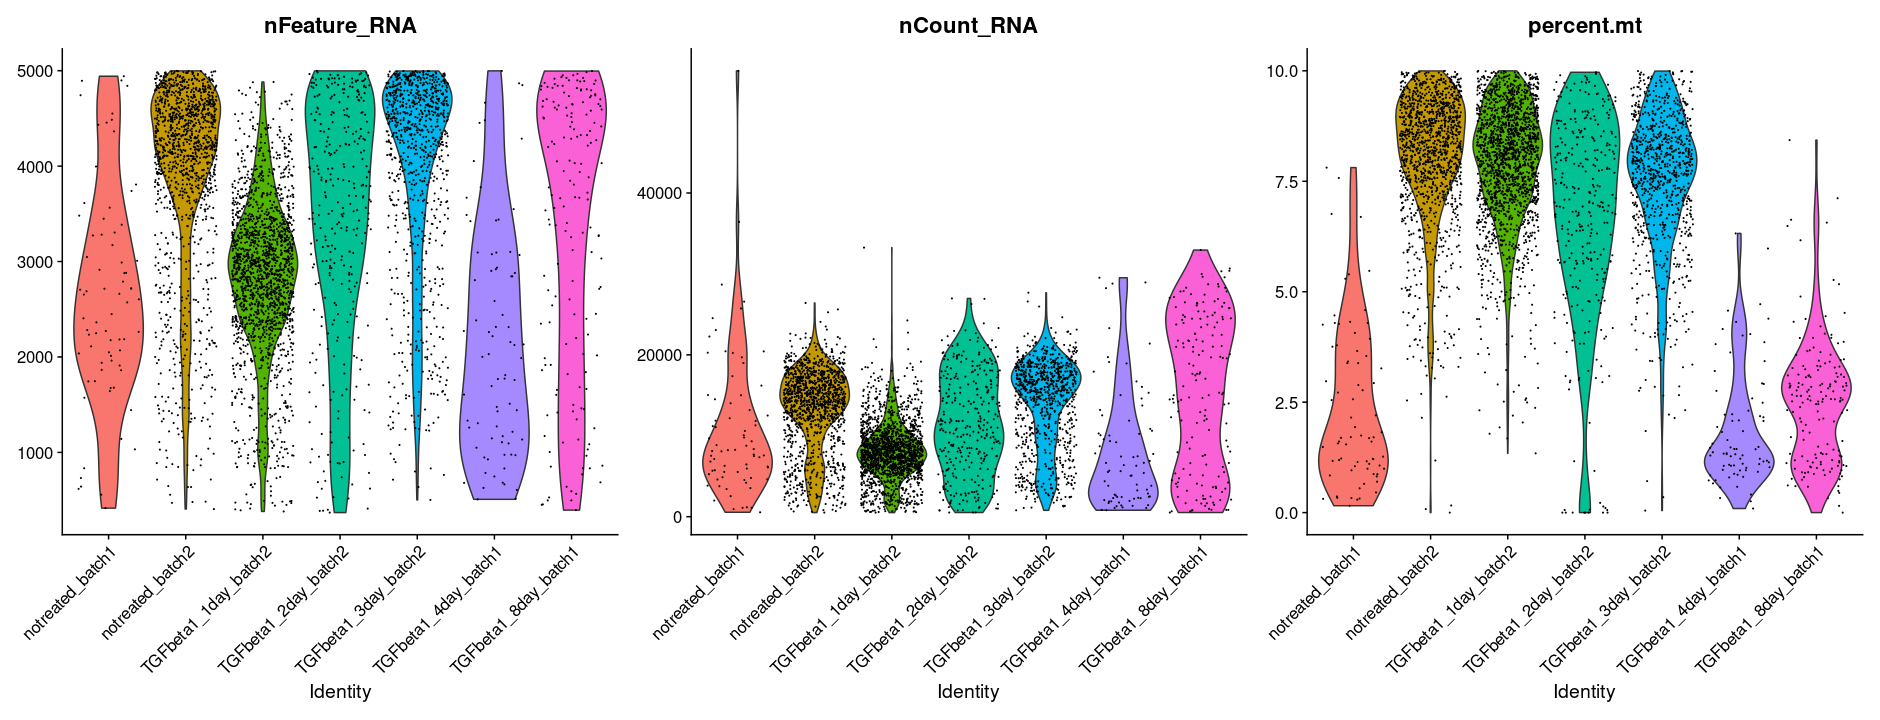
\includegraphics[width=0.75\linewidth]{aposQC.png}
%     \caption{Métricas de Controle de Qualidade Após Filtro}
%     \label{fig:enter-label}
% \end{figure}

% \begin{figure}
%     \centering
%     \includegraphics[width=0.75\linewidth]{GraficosdeDispersãoCountMTFullDay.png}
%     \caption{Distribuição Counts x Genes Mitocondriais}
%     \label{fig:enter-label}
% \end{figure}

% \begin{figure}
%     \centering
%     \includegraphics[width=0.75\linewidth]{GraficosdeDispersãoCountFeatureFullDay.png}
%     \caption{Distribuição Counts x Features}
%     \label{fig:enter-label}
% \end{figure}

% \begin{figure}
%     \centering
%     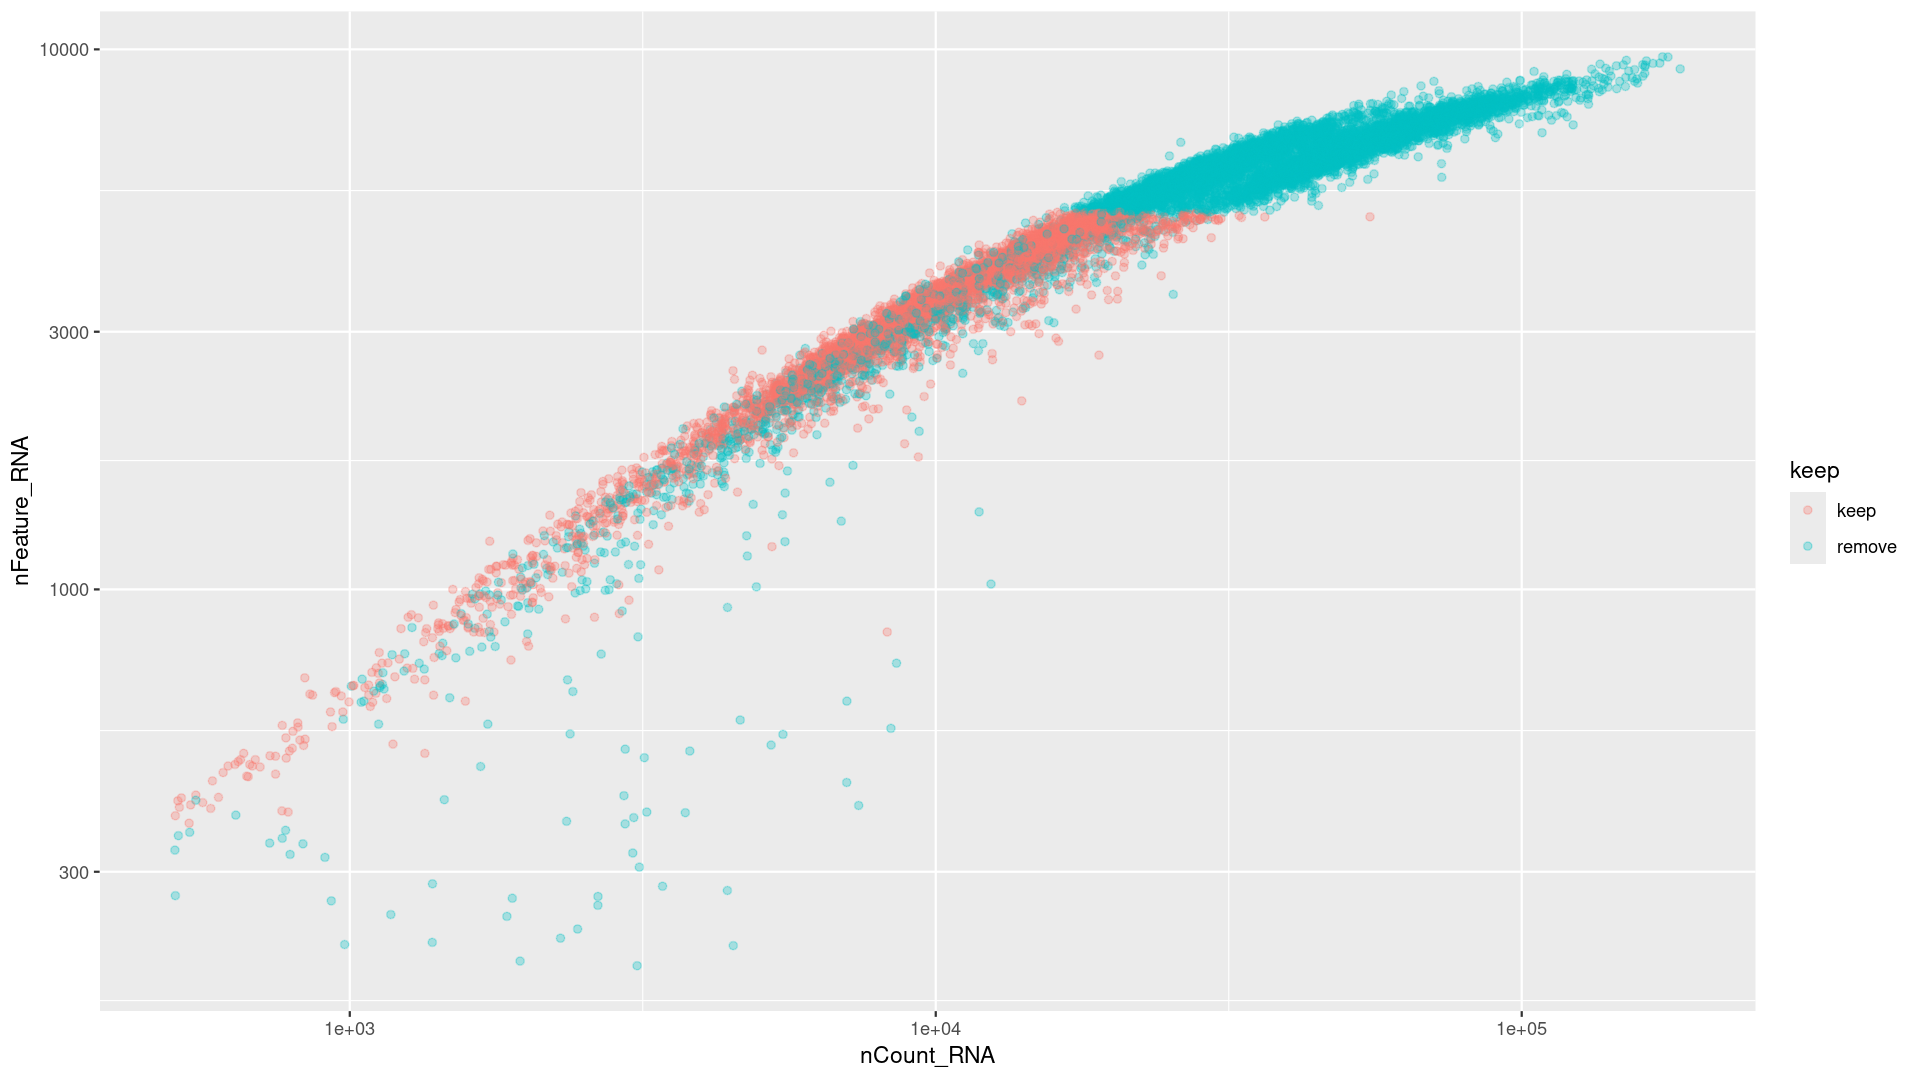
\includegraphics[width=0.75\linewidth]{keepRemoveQC.png}
%     \caption{Distribuição - Keep x Remove}
%     \label{fig:enter-label}
% \end{figure}

% \begin{figure}
%     \centering
%     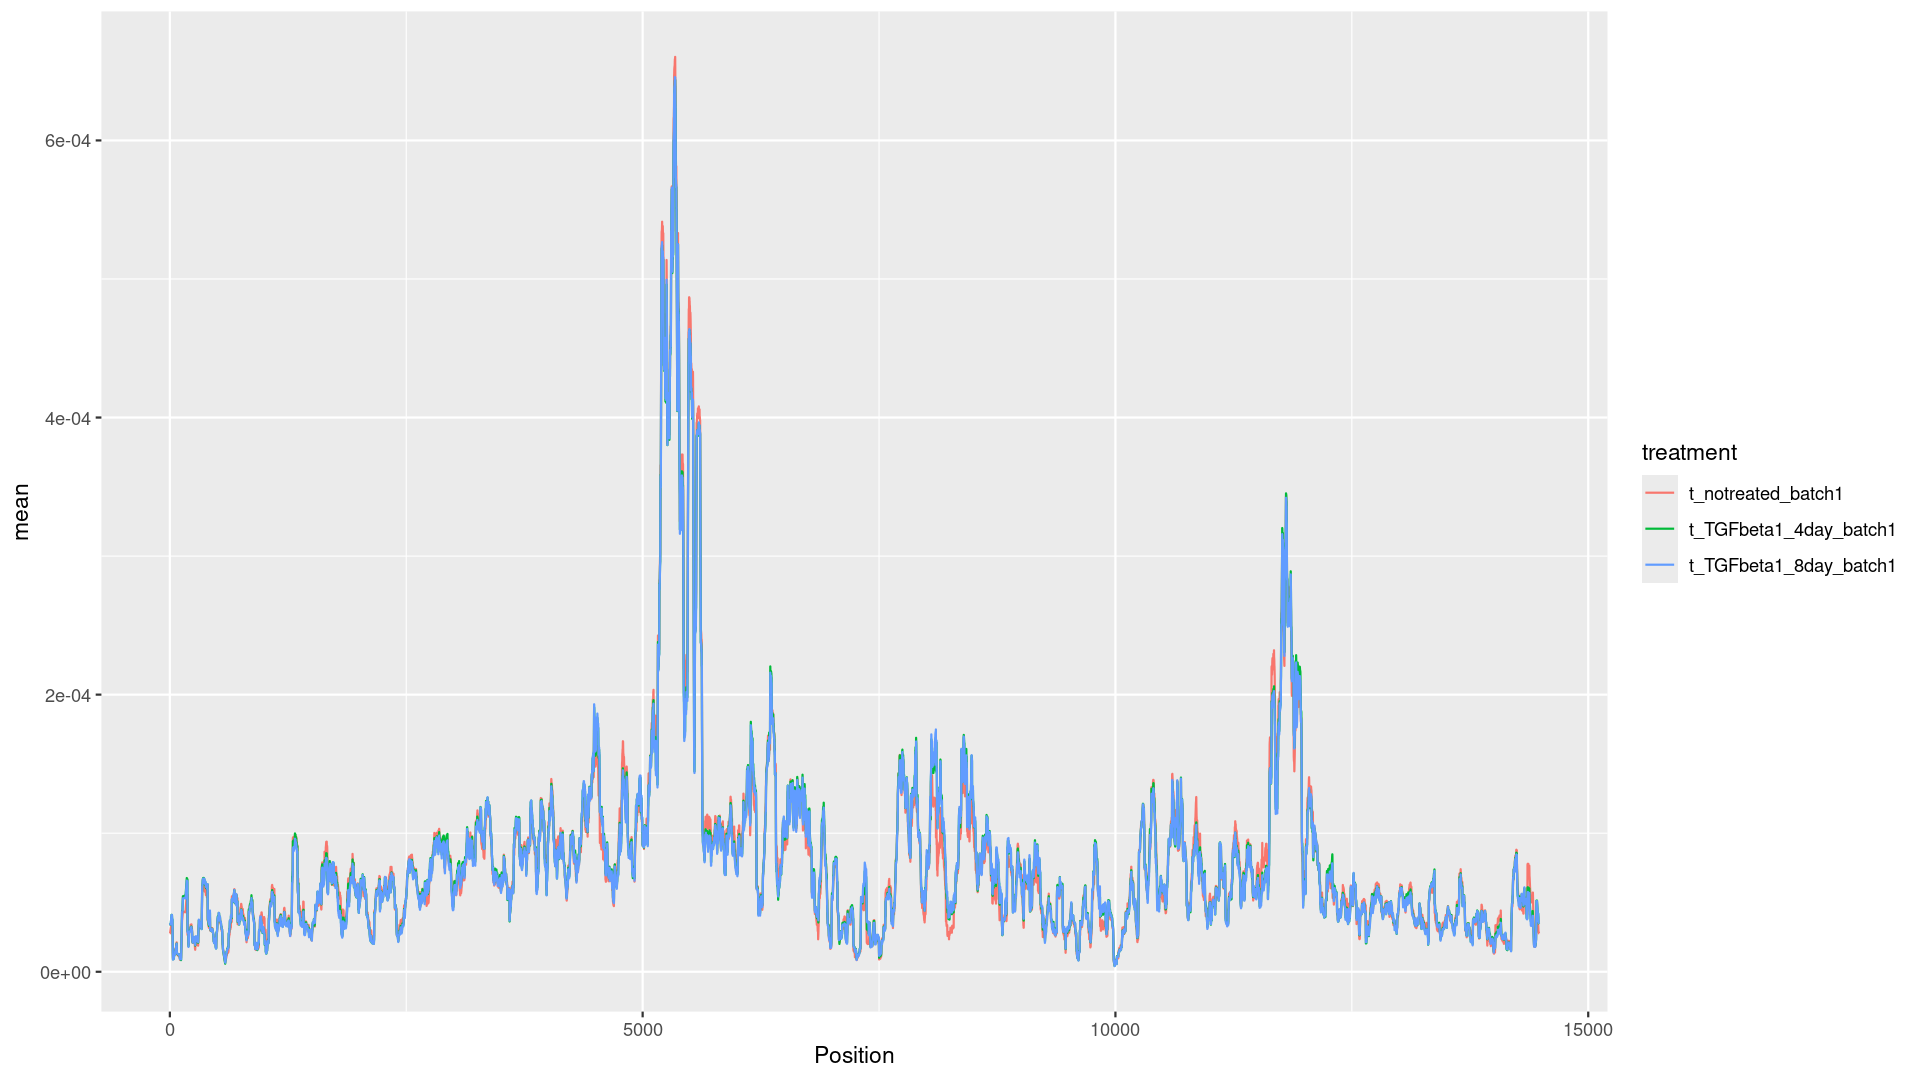
\includegraphics[width=0.75\linewidth]{MeanVariationInFunctionInThePositionProtein_batch1.png}
%     \caption{Variação Média da Expressão das Proteínas - Batch 1}
%     \label{fig:enter-label}
% \end{figure}

% \begin{figure}
%     \centering
%     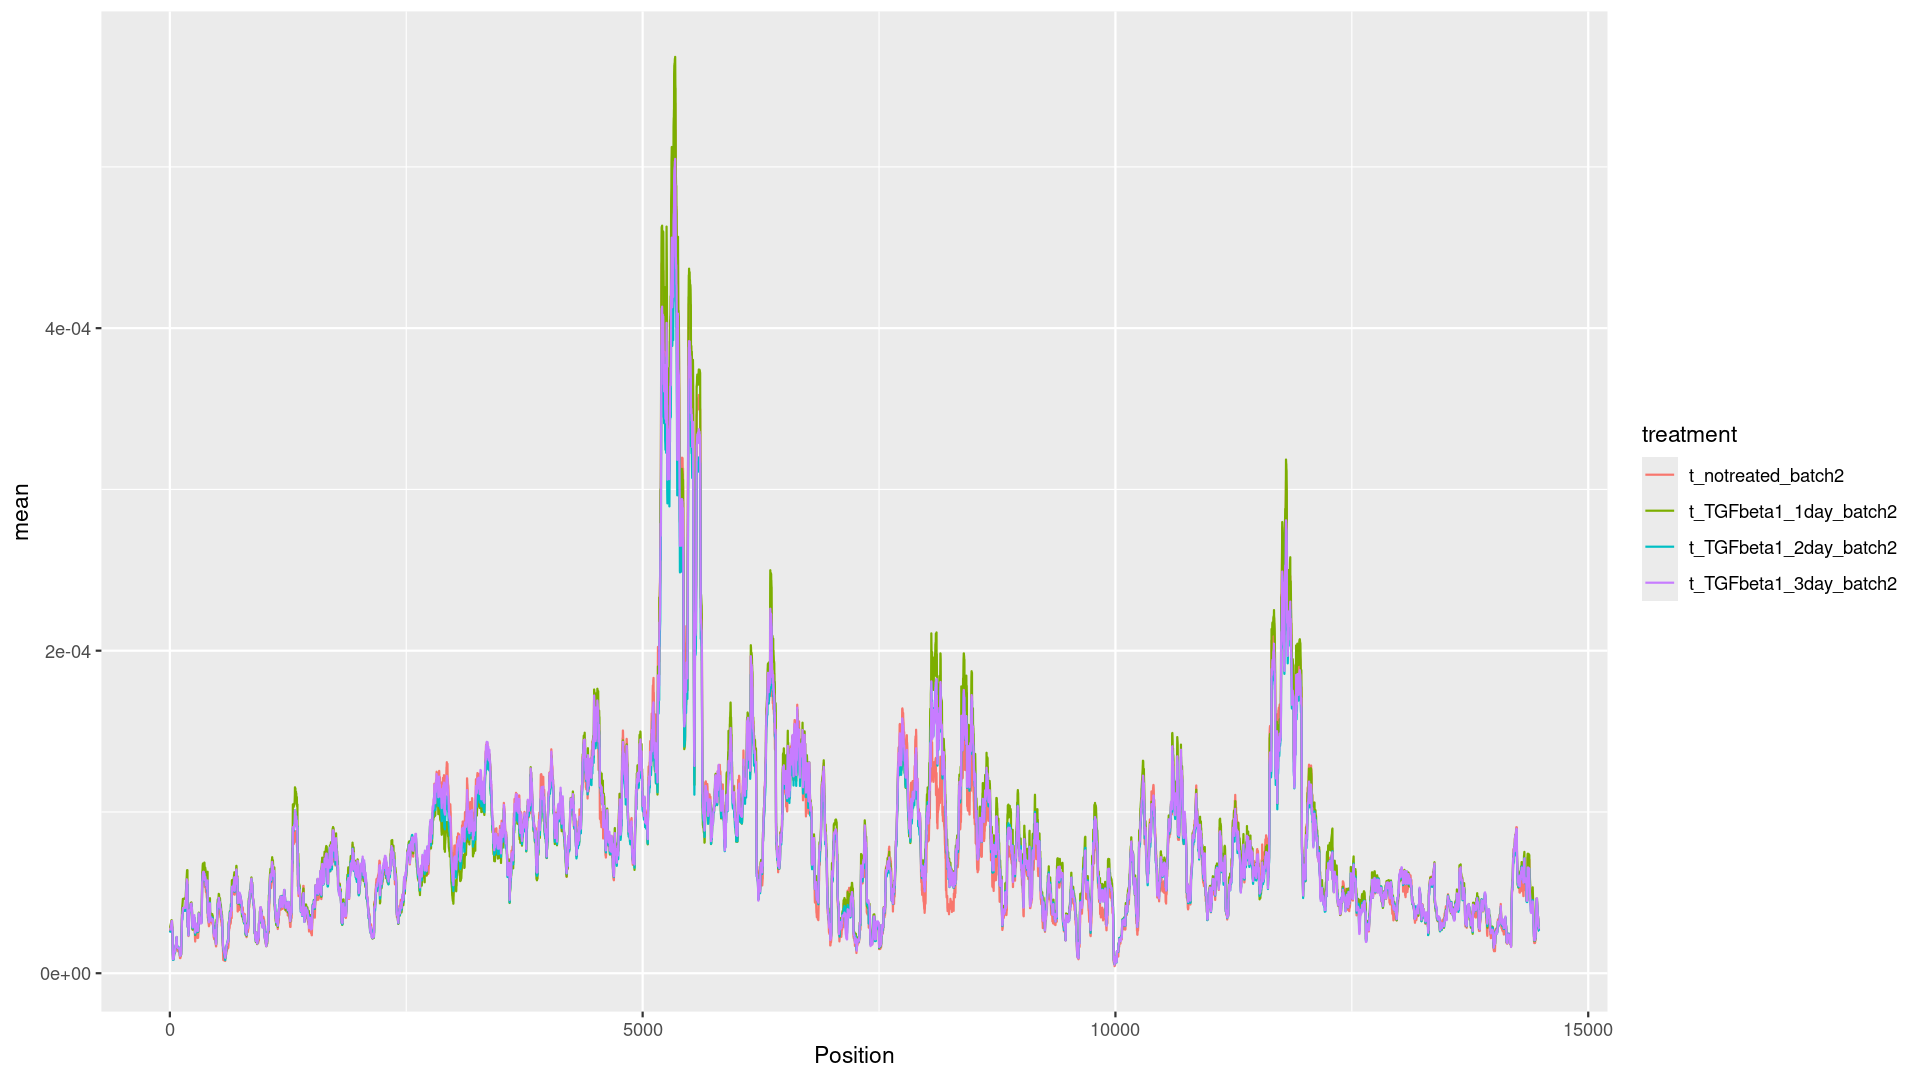
\includegraphics[width=0.75\linewidth]{MeanVariationInFunctionInThePositionProtein_batch2.png}
%     \caption{Variação Média da Expressão das Proteínas - Batch 2}
%     \label{fig:enter-label}
% \end{figure}

% \begin{figure}
%     \centering
%     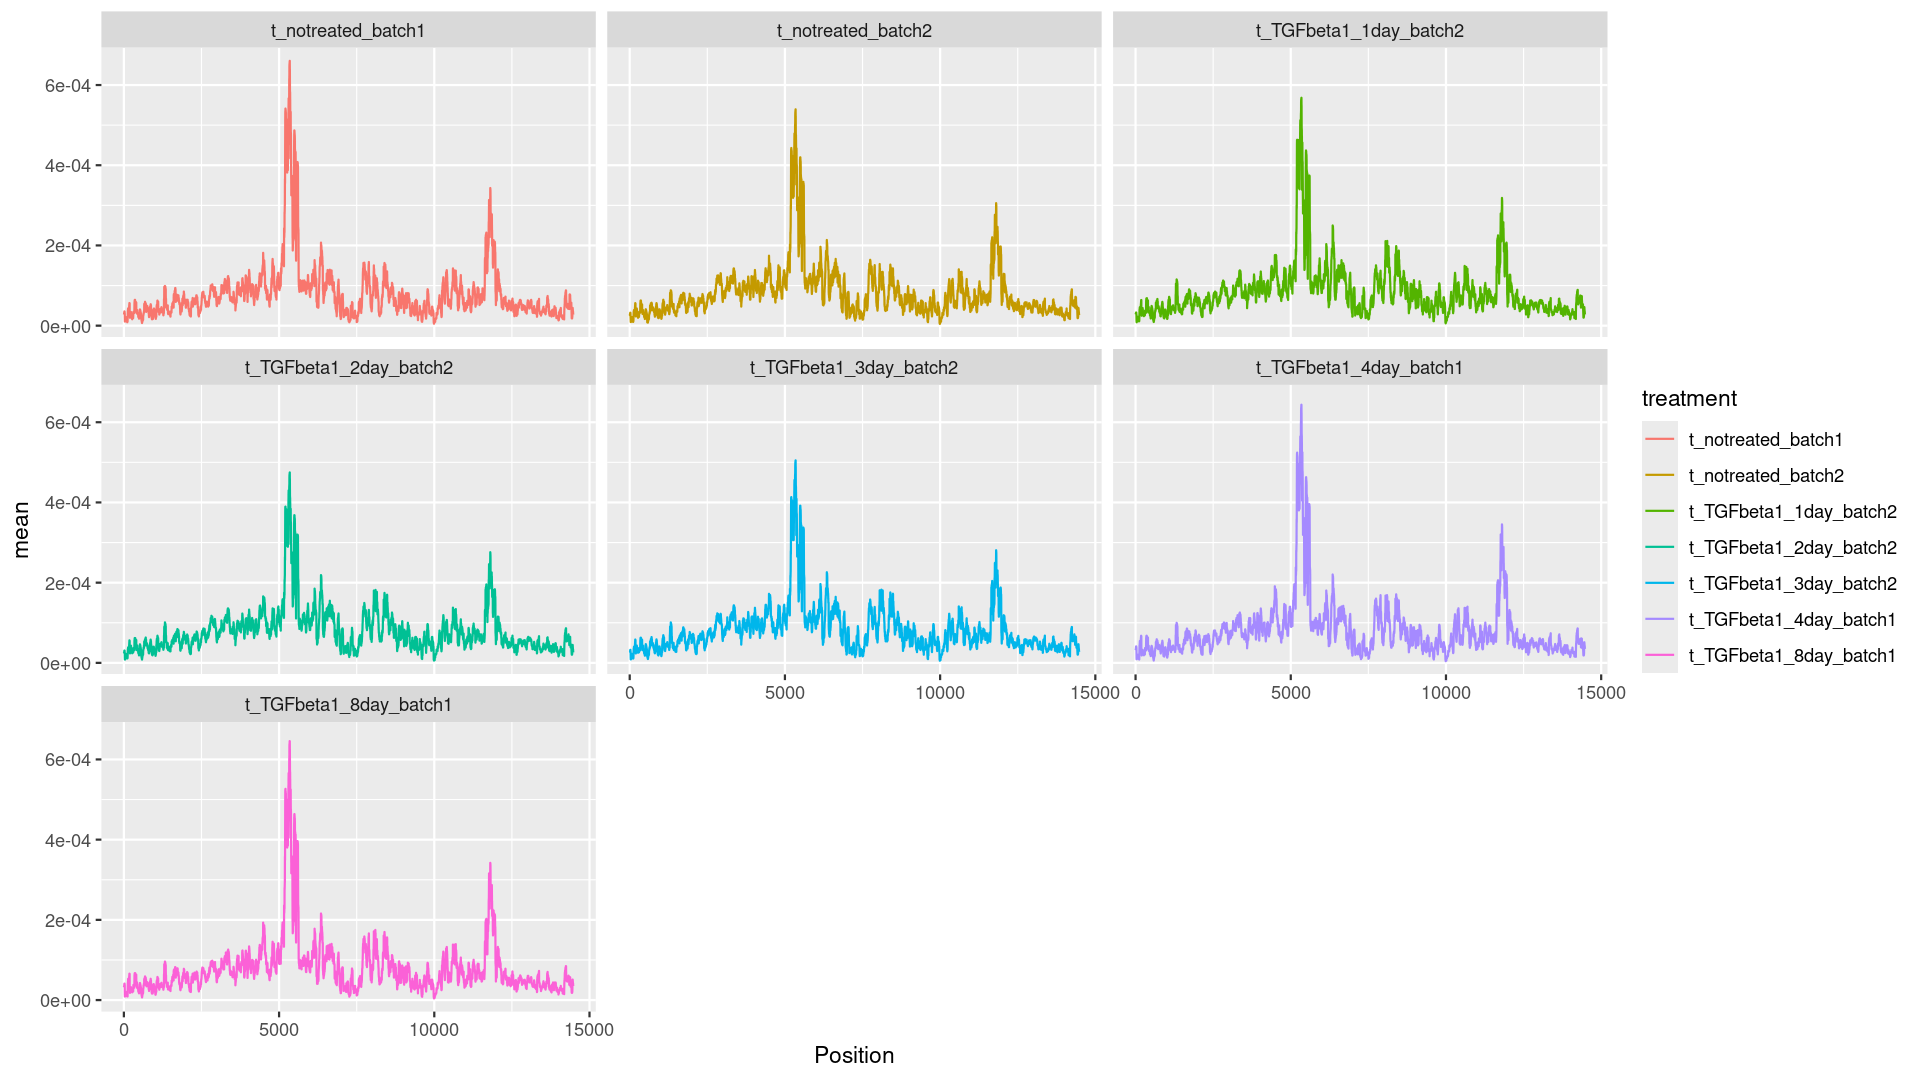
\includegraphics[width=0.75\linewidth]{MeanVariationInFunctionInThePositionProtein.png}
%     \caption{Variação Média da Expressão das Proteínas - Sete Dias}
%     \label{fig:enter-label}
% \end{figure}

% \begin{figure}
%     \centering
%     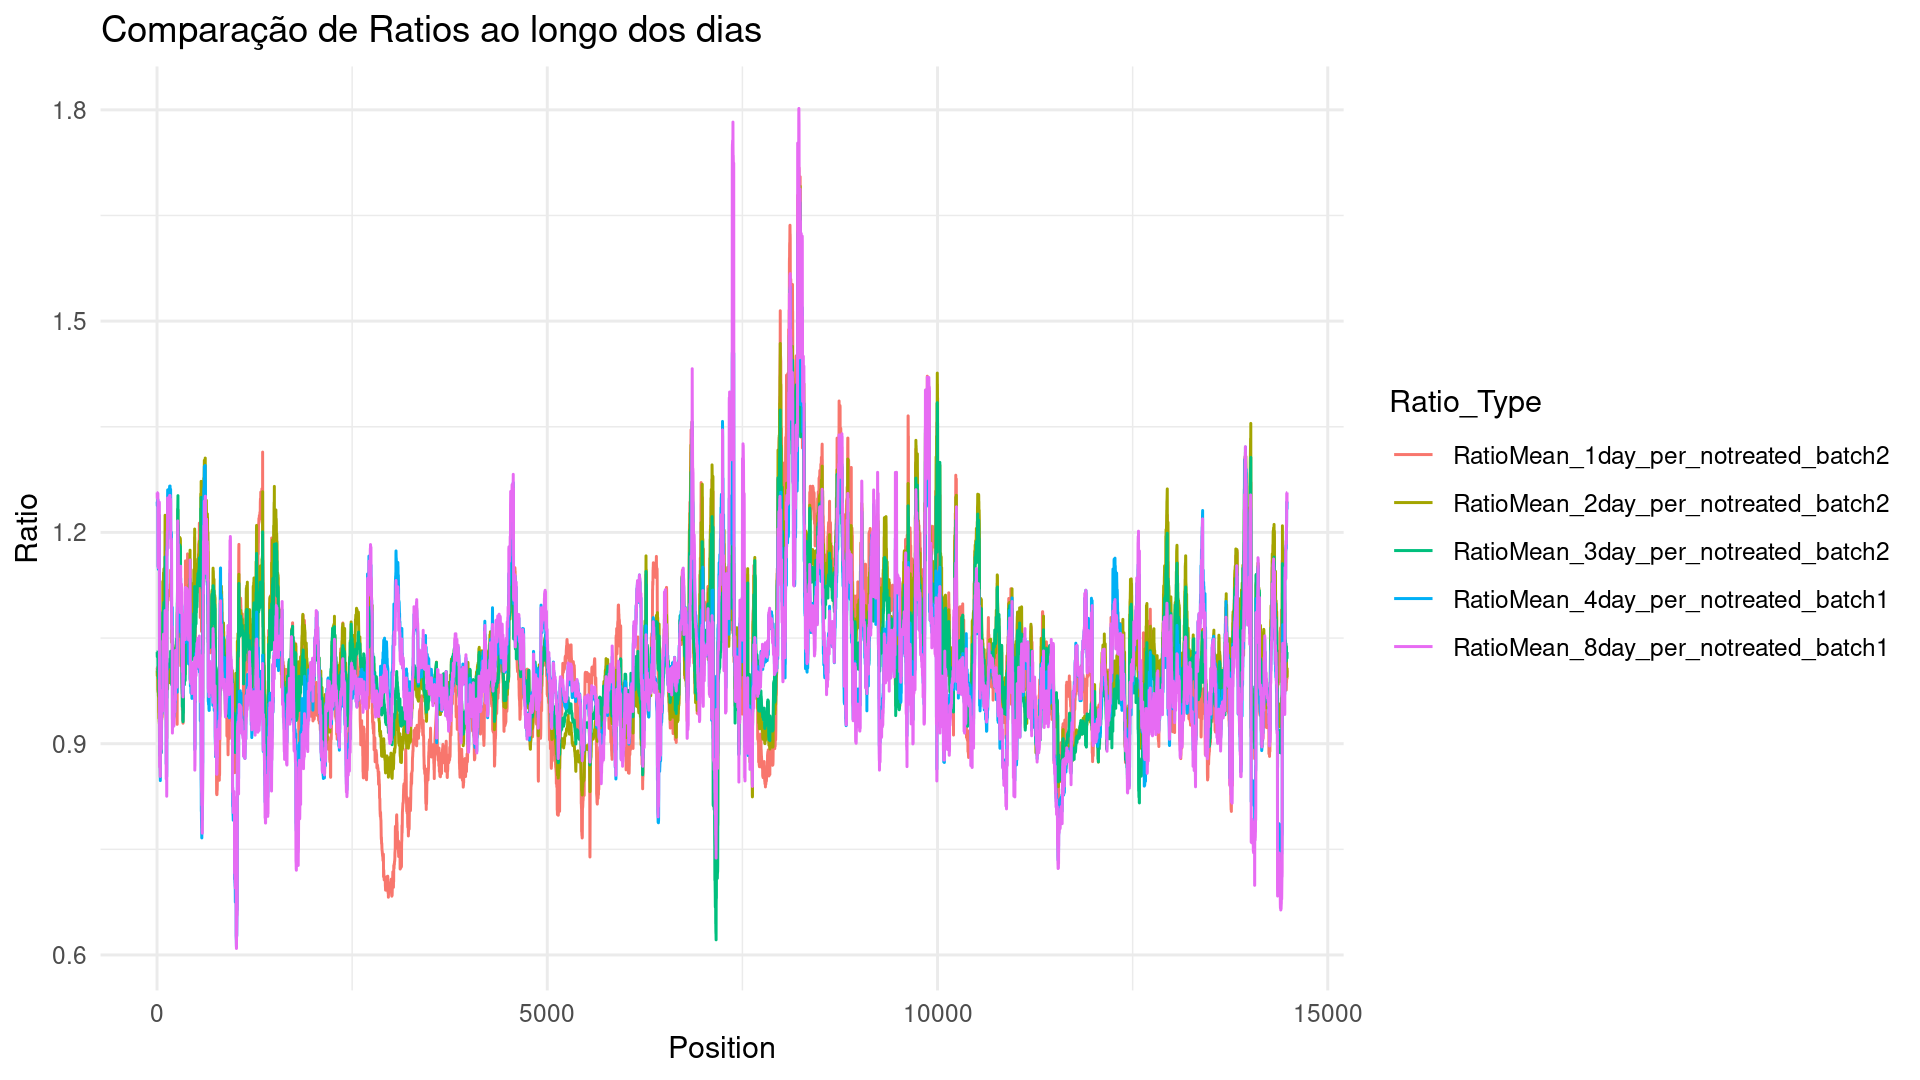
\includegraphics[width=0.75\linewidth]{MeanRatioPerPositionProtein.png}
%      \caption{Razão Média de Cada Dia em Relação do Notreated de Cada Lote.}
%     \label{fig:enter-label}
% \end{figure}

% \begin{figure}
%     \centering
%     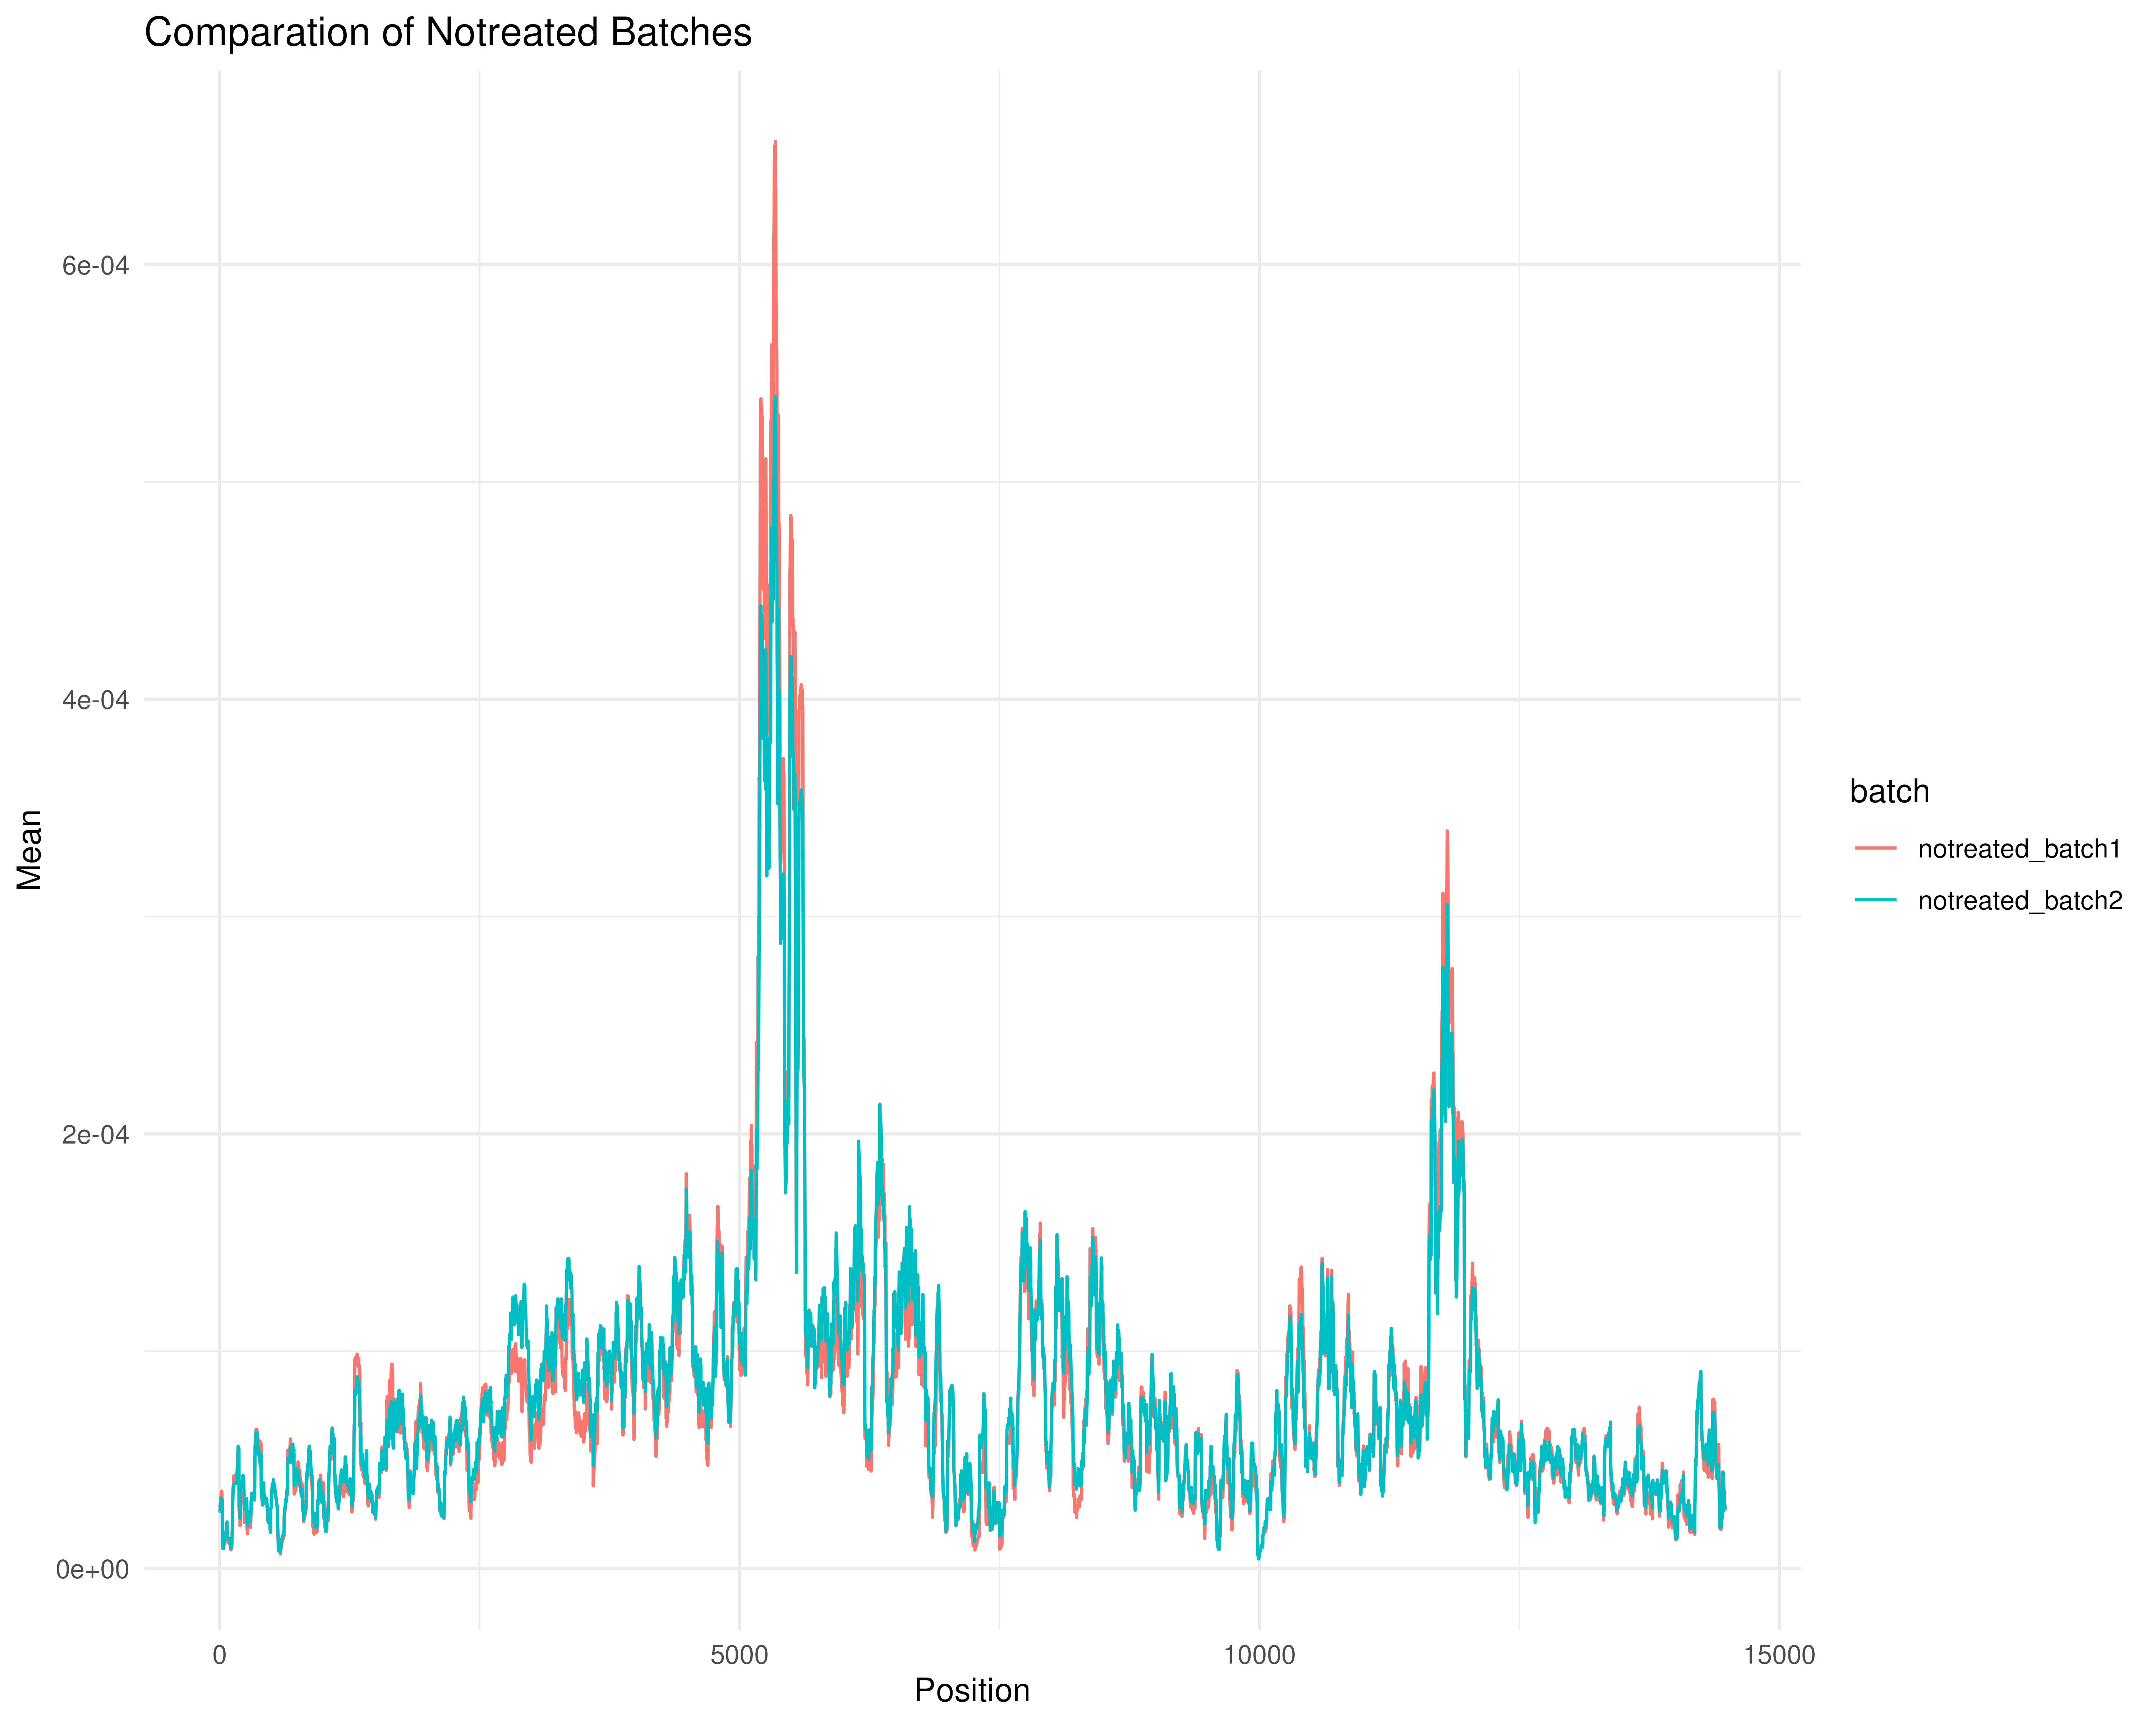
\includegraphics[width=0.75\linewidth]{ComparationOfNotreatedBatchesMean_GGSAVE.png}
%     \caption{Comparativo Entre Médias dos Notreated.}
%     \label{fig:enter-label}
% \end{figure}


\subsection{Normalização dos Dados de Expressão Gênica}

A normalização dos dados de \textit{Single-Cell RNA-seq} foi realizada utilizando o método de contagem total (\textit{Total Count Normalization - TCN}). Esse método ajusta as contagens brutas para minimizar viés devido a diferenças no número total de transcritos sequenciados por célula.

Dado um conjunto de dados de expressão gênica representado por uma matriz $X \in \mathbb{R}^{m \times n}$, onde $m$ é o número de genes e $n$ o número de células, a contagem normalizada de um gene $g$ em uma célula $c$ foi calculada como:

\begin{equation}
    X'_{g,c} = \frac{X_{g,c}}{\sum_{g=1}^{m} X_{g,c}} \times 10^6
\end{equation}

onde $X_{g,c}$ é a contagem bruta do gene $g$ na célula $c$, $\sum_{g=1}^{m} X_{g,c}$ representa o total de leituras da célula $c$ e o fator de escala $10^6$ é utilizado para converter os valores em Transcripts Per Million (TPM), facilitando a interpretação.

\subsection{Correção de Efeitos de Lote}

Os dados foram gerados em dois lotes experimentais distintos, e a correção de efeitos de lote (\textit{batch effect correction}) foi necessária para garantir comparabilidade entre os conjuntos de dados. Para isso, foi aplicada uma correção baseada na normalização por média de expressão gênica entre os lotes.

Definindo a expressão média de um gene $g$ no lote $b$ como:

\begin{equation}
    \bar{X}_{g,b} = \frac{1}{n_b} \sum_{c=1}^{n_b} X'_{g,c}
\end{equation}

onde $n_b$ é o número de células no lote $b$, a correção foi aplicada ajustando cada expressão gênica em relação à média global dos lotes:

\begin{equation}
    X''_{g,c} = X'_{g,c} \times \frac{\bar{X}_g}{\bar{X}_{g,b}}
\end{equation}

onde $\bar{X}_g$ é a média global de expressão do gene $g$ considerando todos os lotes. Esse procedimento assegura que diferenças observadas na expressão gênica reflitam variação biológica real e não artefatos técnicos provenientes dos diferentes lotes experimentais.



\subsection{Método Transcriptogramer\cite{morais}}

O \textit{Transcriptogramer} é um método de análise transcricional que projeta dados de expressão gênica em uma lista ordenada de proteínas, permitindo a identificação de agrupamentos funcionais e a análise da regulação gênica no contexto de uma rede de interação proteína-proteína (\textit{PPI}). Esse método possibilita a detecção de padrões diferenciais de expressão considerando relações funcionais entre genes.

\subsubsection{Entradas do Método}

São esperados quatro tipos principais de entrada:
\begin{itemize}
    \item \textbf{Rede de interação proteína-proteína (PPI)} – Representada por um grafo onde os nós correspondem a proteínas e as arestas indicam interações conhecidas.
    \item \textbf{Lista ordenada de proteínas} – Uma ordenação inicial arbitrária das proteínas, que será otimizada pelo método.
    \item \textbf{Valores de expressão gênica} – Obtidos por técnicas como RNA-Seq ou Microarray.
    \item \textbf{Dicionário de mapeamento} – Relaciona os valores de expressão gênica às proteínas correspondentes.
\end{itemize}

Além disso, o método pode aceitar diretamente dados brutos de RNA-Seq e Microarray para processamento.

\subsubsection{Ordenação das Proteínas e Algoritmo CFM}

Inicialmente, a lista de proteínas é disposta em uma ordem arbitrária nos dois eixos da matriz de interações. O método utiliza o \textbf{Algoritmo CFM (Cost Function Minimization)} para otimizar essa ordenação, aproximando interações da diagonal principal. O processo ocorre iterativamente por meio de:


\begin{itemize}
    \item Trocas aleatórias entre linhas e colunas.
    \item Cálculo do custo associado à nova configuração.
    \begin{itemize}
        \item Se o custo for reduzido, a troca é aceita.
        \item Se o custo aumentar, o método de \textit{Simulated Annealing} avalia a aceitação de configurações piores para evitar mínimos locais.
    \end{itemize}
\end{itemize}

\begin{figure}
    \centering
    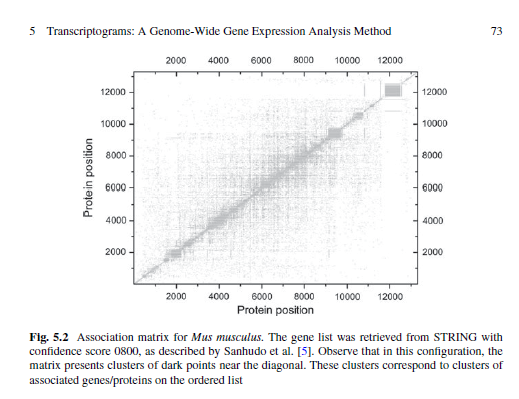
\includegraphics[width=0.75\linewidth]{Transcriptograma.png}
    \caption{Exemplo de transcriprograma com ordenadeção final e visualização clara de agrupamentos. \cite{deAlmeida2020}}
    \label{fig:enter-label}
\end{figure}

O custo da configuração é definido como:

\begin{equation}
    CFM = \sum_{i,j} A_{i,j} \cdot d(i,j),
\end{equation}

onde $A_{i,j}$ representa a matriz de adjacência da rede de interações e $d(i,j)$ é a distância euclidiana entre as proteínas $i$ e $j$ na ordenação atual.

Após sucessivas iterações, obtém-se uma configuração otimizada, onde interações estão mais próximas da diagonal principal, refletindo melhor a estrutura funcional da rede.

\subsubsection{Cálculo dos Valores de Expressão}

Os valores de expressão gênica são calculados com base em janelas deslizantes sobre a lista ordenada de proteínas. Para cada gene central $g$, um grupo de genes vizinhos dentro de um raio $r$ é selecionado. Assim, o valor de expressão normalizado para o gene $g$ é dado por:

\begin{equation}
    E_g = \frac{1}{2r+1} \sum_{i=g-r}^{g+r} e_i,
\end{equation}

onde $e_i$ é a expressão do gene $i$. Se tivermos uma lista ordenada com $N$ genes e um raio $r$, cada gene terá sua expressão recalculada com base em uma janela de $2r+1$ genes. Para um raio de $r = 30$, cada média envolverá 61 genes.

\subsubsection{Identificação de Genes Diferencialmente Expressos}

Para detectar genes diferencialmente expressos (\textit{DEGs - Differentially Expressed Genes}), foram comparadas diferentes condições experimentais. Os genes com variação significativa foram classificados em:
\begin{itemize}
    \item \textbf{Upregulated} – Genes com aumento significativo de expressão em relação ao controle.
    \item \textbf{Downregulated} – Genes com redução significativa de expressão.
\end{itemize}

A avaliação estatística foi realizada utilizando testes de hipóteses apropriados, como o teste $t$ de Student ou o teste de Mann-Whitney, dependendo da distribuição dos dados.

\subsubsection{Enriquecimento Funcional e Visualização dos Resultados}

Os genes diferencialmente expressos foram analisados para determinar sua relevância biológica por meio de técnicas de \textbf{enriquecimento funcional}, que permitem associar conjuntos de genes a processos biológicos, funções moleculares e vias metabólicas específicas. O enriquecimento foi conduzido utilizando bancos de dados como \textit{Gene Ontology} (GO) e \textit{KEGG Pathways}, proporcionando uma visão mais abrangente dos processos biológicos alterados.

Os resultados foram representados graficamente para melhor interpretação dos padrões diferenciais de expressão e das associações funcionais. Os principais métodos de visualização incluíram:
\begin{itemize}
    \item \textbf{Heatmaps} – Para representar a variação da expressão gênica ao longo da lista ordenada.
    \item \textbf{Redes funcionais} – Para destacar conexões entre genes diferencialmente expressos.
    \item \textbf{Gráficos de enriquecimento} – Para ilustrar processos biológicos significativamente afetados.
\end{itemize}

A combinação dessas abordagens permitiu uma análise detalhada da expressão gênica em um contexto funcional, fornecendo insights relevantes sobre a regulação gênica nos diferentes estados biológicos analisados.

\begin{figure}
    \centering
    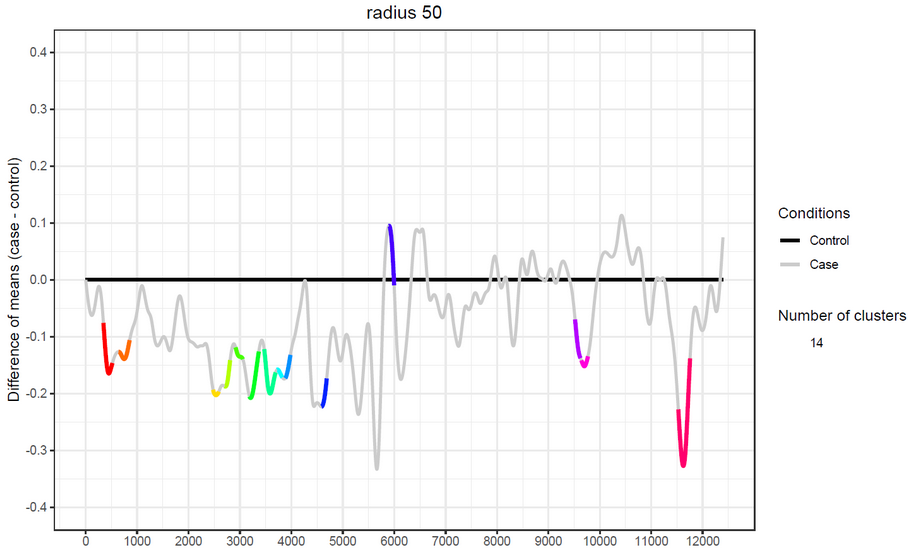
\includegraphics[width=0.75\linewidth]{transcriptogramer.png}
    \caption{Exemplo de Gráfico de Expressão Diferencial do Transcriptogra \cite{morais}}
    \label{fig:enter-label}
\end{figure}

\subsection{Expectativas e Objetivos}

Este estudo busca aplicar o método \textit{Transcriptogramer}, aliado a dados de expressão gênica de \textit{single-cell RNA-Seq} (\textit{scRNA-Seq}), para analisar a dinâmica da transição epitélio-mesenquimal (\textit{EMT - Epithelial-Mesenchymal Transition}). A transição EMT desempenha um papel fundamental em processos biológicos como desenvolvimento embrionário, cicatrização de feridas e progressão tumoral.  

Espera-se que, por meio do \textit{Transcriptogramer}, seja possível representar visualmente a expressão gênica em células individuais ao longo dessa transição e identificar estágios intermediários do processo. Além disso, o método permitirá a detecção de agrupamentos funcionais e a análise de padrões diferenciais de expressão entre diferentes estados celulares. A utilização de dados \textit{single-cell} representa um avanço significativo na aplicação do \textit{Transcriptogramer}, ampliando sua capacidade de análise em níveis mais refinados de heterogeneidade celular.

\subsection{Células MCF10A: Um Modelo para Estudo da Transição EMT}

As células \textbf{MCF10A} são uma linha celular humana derivada de tecido epitelial mamário não canceroso, amplamente utilizada como modelo \textit{in vitro} para estudar processos biológicos associados à progressão do câncer de mama. Por serem células epiteliais não tumorais, as MCF10A representam um excelente sistema para investigar mecanismos moleculares da transição epitélio-mesenquimal, permitindo a análise de estados celulares distintos, desde um fenótipo epitelial até formas parcialmente ou totalmente mesenquimais.  

Neste estudo, dados de \textit{scRNA-Seq} de células MCF10A serão explorados com o \textit{Transcriptogramer} para identificar assinaturas gênicas associadas a diferentes estágios da EMT, proporcionando uma visão mais detalhada sobre a heterogeneidade transcricional durante esse processo. Esse enfoque permitirá compreender melhor os mecanismos regulatórios subjacentes e poderá fornecer novas perspectivas sobre alvos terapêuticos relacionados à plasticidade celular no câncer de mama.


\subsection{Lotes vs Tempo - Suspensões Unicelulares de Células MCF10A}

A análise transcricional das células MCF10A foi realizada a partir de suspensões unicelulares coletadas em diferentes tempos experimentais. No entanto, os dados foram gerados utilizando diferentes versões do sistema de captura de RNA da \textit{10x Genomics}: os kits v2 e v3. Essa diferença técnica resultou na formação de dois lotes distintos de dados, cuja comparabilidade requer normalização adequada.

\subsubsection{Principais Diferenças entre os Kits v2 e v3}

Os kits v2 e v3 representam versões aprimoradas do sistema de captura e amplificação de RNA da \textit{10x Genomics}. Suas diferenças impactam diretamente a sensibilidade, a cobertura e a estrutura dos dados gerados. As principais melhorias incluem:

\paragraph{Sensibilidade Aprimorada no v3}  
O kit v3 possui maior eficiência na captura de RNA, permitindo a detecção de um maior número de genes por célula em comparação com o v2. Isso se deve a aprimoramentos no design dos primers e na eficiência da transcrição reversa.

\paragraph{Maior Cobertura de Sequenciamento}  
A versão v3 permite a recuperação de mais transcritos únicos (\textit{Unique Molecular Identifiers} - UMIs), reduzindo o viés e aumentando a precisão da quantificação gênica.

\paragraph{Alterações na Estrutura do cDNA}  
O protocolo do kit v3 introduziu mudanças na sequência dos oligonucleotídeos utilizados na captura e amplificação do cDNA, otimizando a eficiência da reação e melhorando a fidelidade da quantificação.

\paragraph{Impacto na Comparação de Dados}  
Como os kits v2 e v3 possuem diferenças estruturais e metodológicas, os dados gerados por cada versão podem apresentar variações técnicas que dificultam a comparação direta. Para garantir que as diferenças observadas sejam biológicas e não técnicas, é fundamental aplicar métodos de normalização e correção de efeitos de lote.

%%%%%% TRANSCRIPTOGRAMA PARA R0 E R30 %%%%%%

\subsection{Análise com Diferentes Valores de Raio}

Para avaliar o impacto do parâmetro de suavização no método \textit{Transcriptogramer}, realizamos análises considerando dois valores distintos de raio: $r = 0$ e $r = 30$. 

\subsubsection{Transcriptograma com Raio 0}
Quando $r = 0$, a expressão gênica é analisada sem qualquer suavização, ou seja, os valores de expressão de cada gene são considerados individualmente sem influência dos seus vizinhos na ordenação. Esse cenário permite uma observação direta das variações de expressão gênica e a identificação de genes diferencialmente expressos (\textit{DEGs}) de forma mais localizada. Contudo, esse método pode ser mais sensível ao ruído biológico e técnico presente nos dados de expressão gênica.

\subsubsection{Transcriptograma com Raio 30}
Ao utilizar $r = 30$, aplicamos um processo de suavização onde cada gene tem seu valor de expressão calculado com base em uma média ponderada considerando seus 30 vizinhos anteriores e posteriores na lista ordenada de proteínas. Essa abordagem reduz a variabilidade local, permitindo a identificação de padrões globais de expressão gênica e agrupamentos funcionais mais evidentes. A suavização facilita a detecção de tendências na regulação gênica e melhora a interpretação biológica ao minimizar flutuações espúrias nos dados.

\subsubsection{Comparação entre os Diferentes Valores de Raio}
A comparação entre os resultados obtidos com $r = 0$ e $r = 30$ possibilitou a identificação de padrões distintos na expressão gênica. Enquanto o raio menor favorece a detecção de variações pontuais e genes diferencialmente expressos com mudanças abruptas, o raio maior fornece uma visão mais integrada da regulação gênica no contexto da rede de interação proteína-proteína. Essa abordagem combinada permite uma análise mais robusta e informativa da expressão gênica nos diferentes estados celulares investigados.

\subsubsection{Análise de Componentes Principais (PCA)}
Para complementar a análise dos transcriptogramas obtidos com $r = 0$ e $r = 30$, realizaremos uma Análise de Componentes Principais (PCA) em ambos os conjuntos de dados. Essa abordagem permitirá visualizar a variação global da expressão gênica e identificar possíveis agrupamentos ou padrões diferenciais de regulação gênica entre os diferentes estados celulares analisados. A PCA facilitará a interpretação dos dados, reduzindo a dimensionalidade e destacando as principais fontes de variação na expressão gênica.

\subsection{Parâmetros da PCA}
Utilizamos o parâmetro \texttt{scale=FALSE}, visto que pretendemos preservar a variação original dos dados, evitando reduzir a importância das variáveis mais informativas. Além disso, como todas as variáveis estão na mesma unidade de medida, a padronização não se faz necessária. Esse ajuste garante que a PCA capture a estrutura inerente dos dados sem distorções artificiais causadas pela normalização.





\begin{figure}
    \centering
    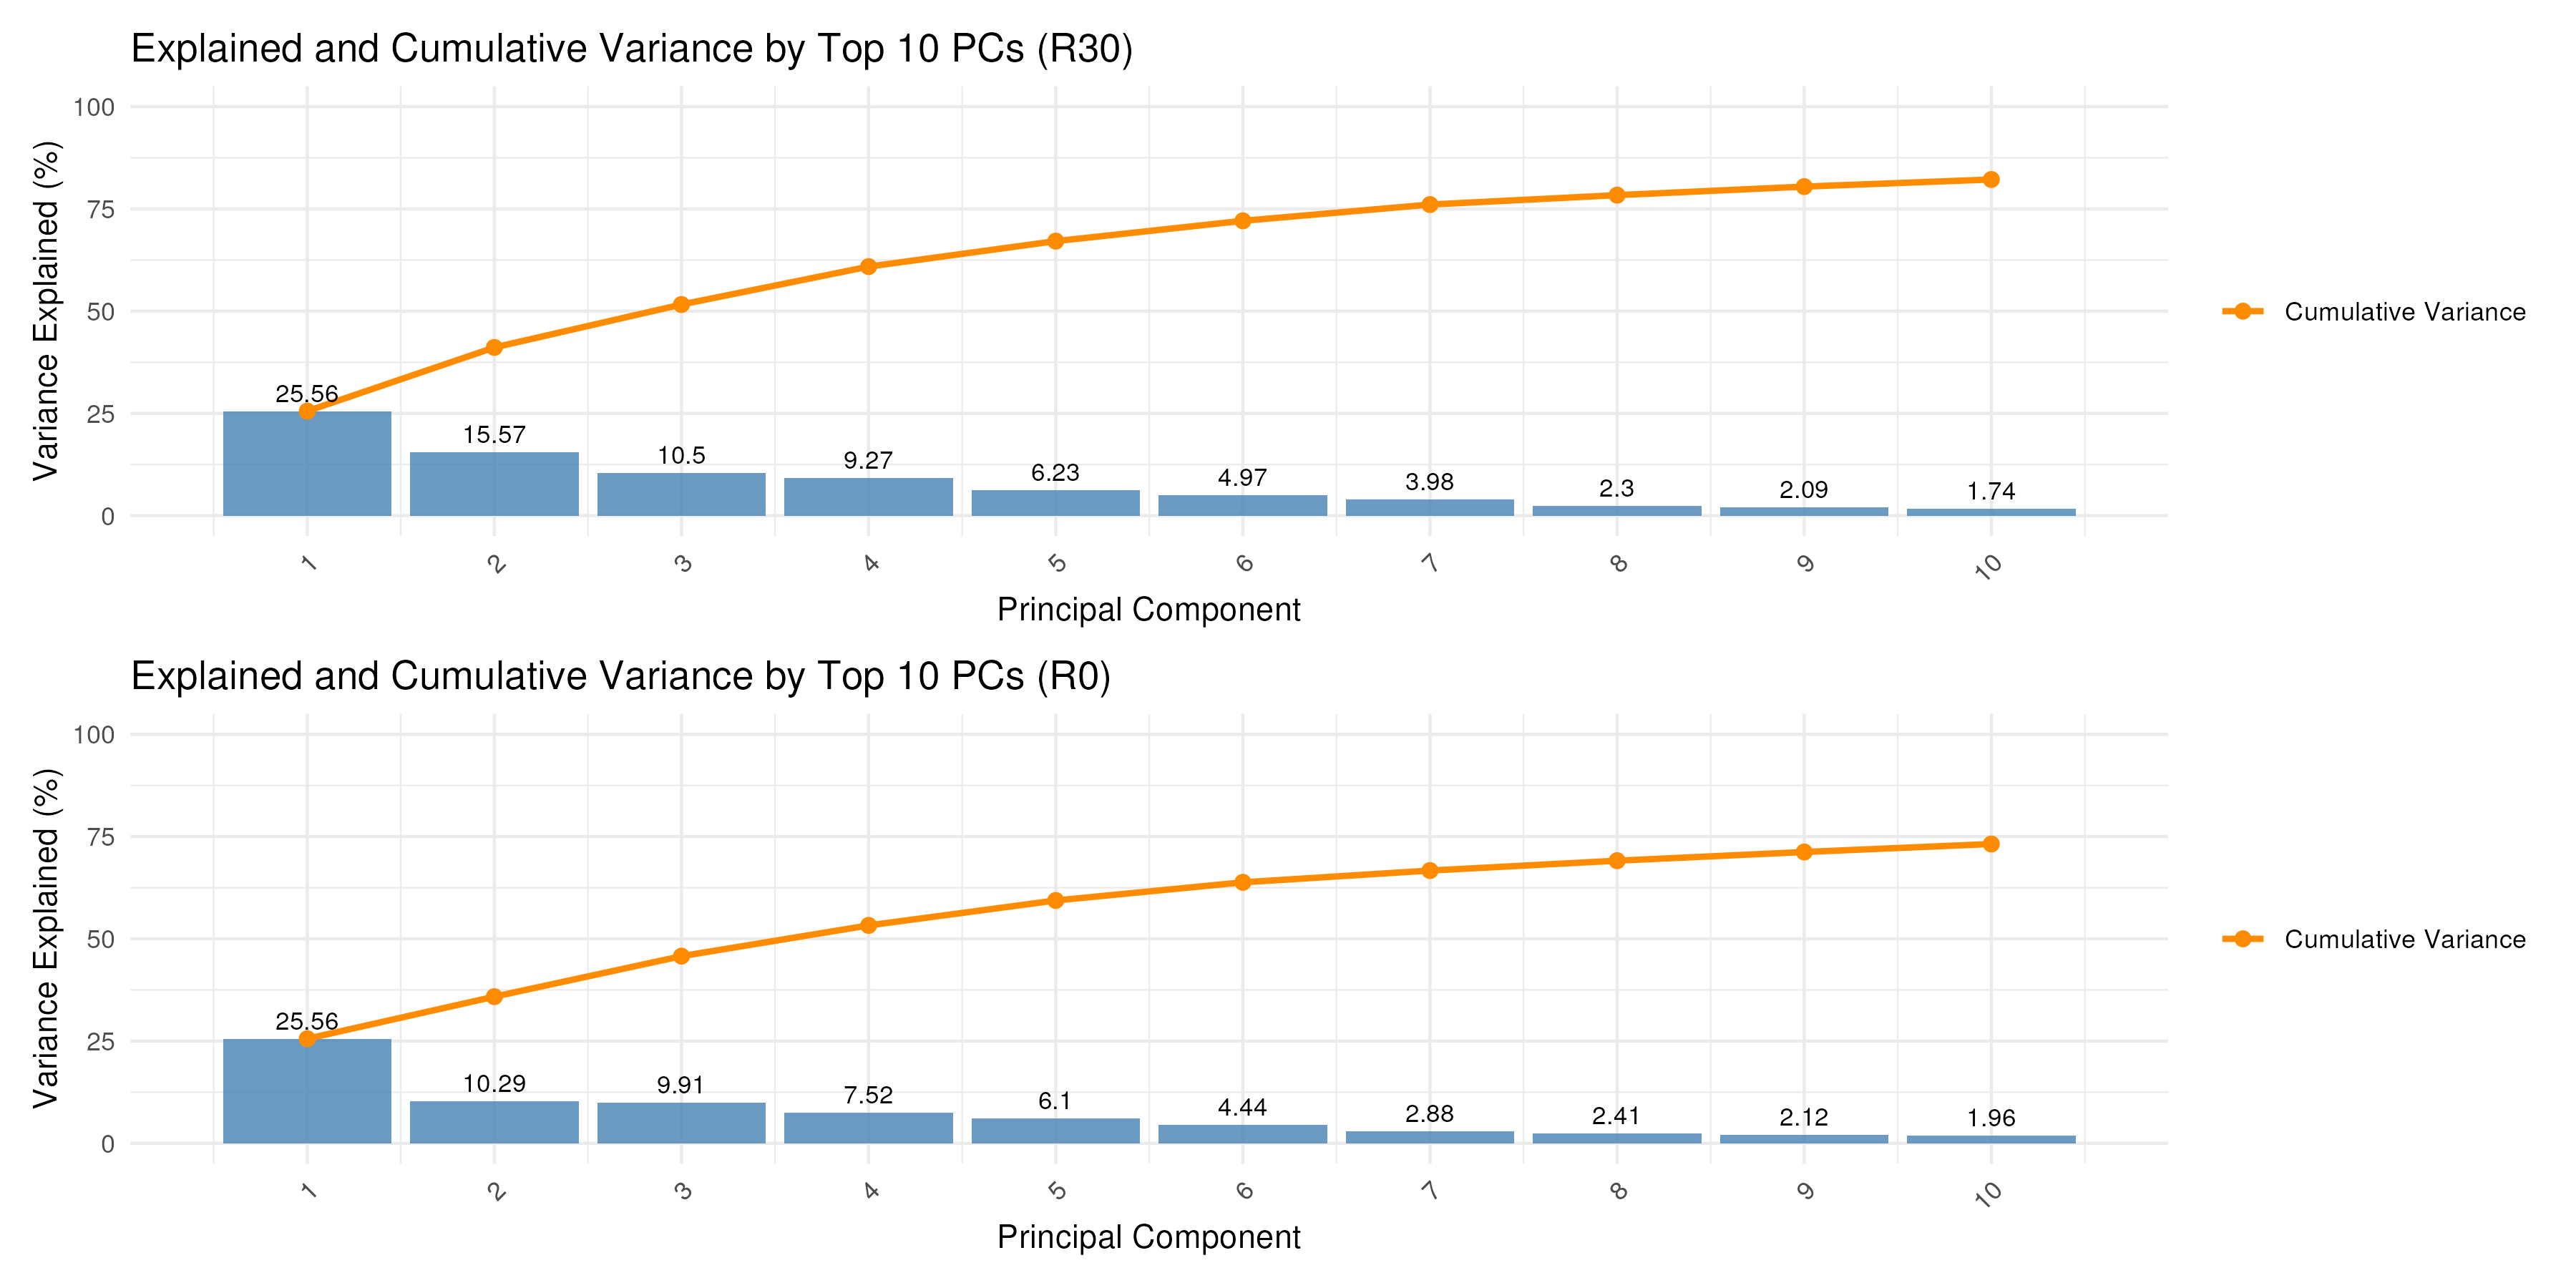
\includegraphics[width=0.75\linewidth]{combined_explained_cumulative_variance_top10.png}
    \caption{Variância de Componentes Principais - R0 e R30}
    \label{fig:enter-label}
\end{figure}

\begin{figure}
    \centering
    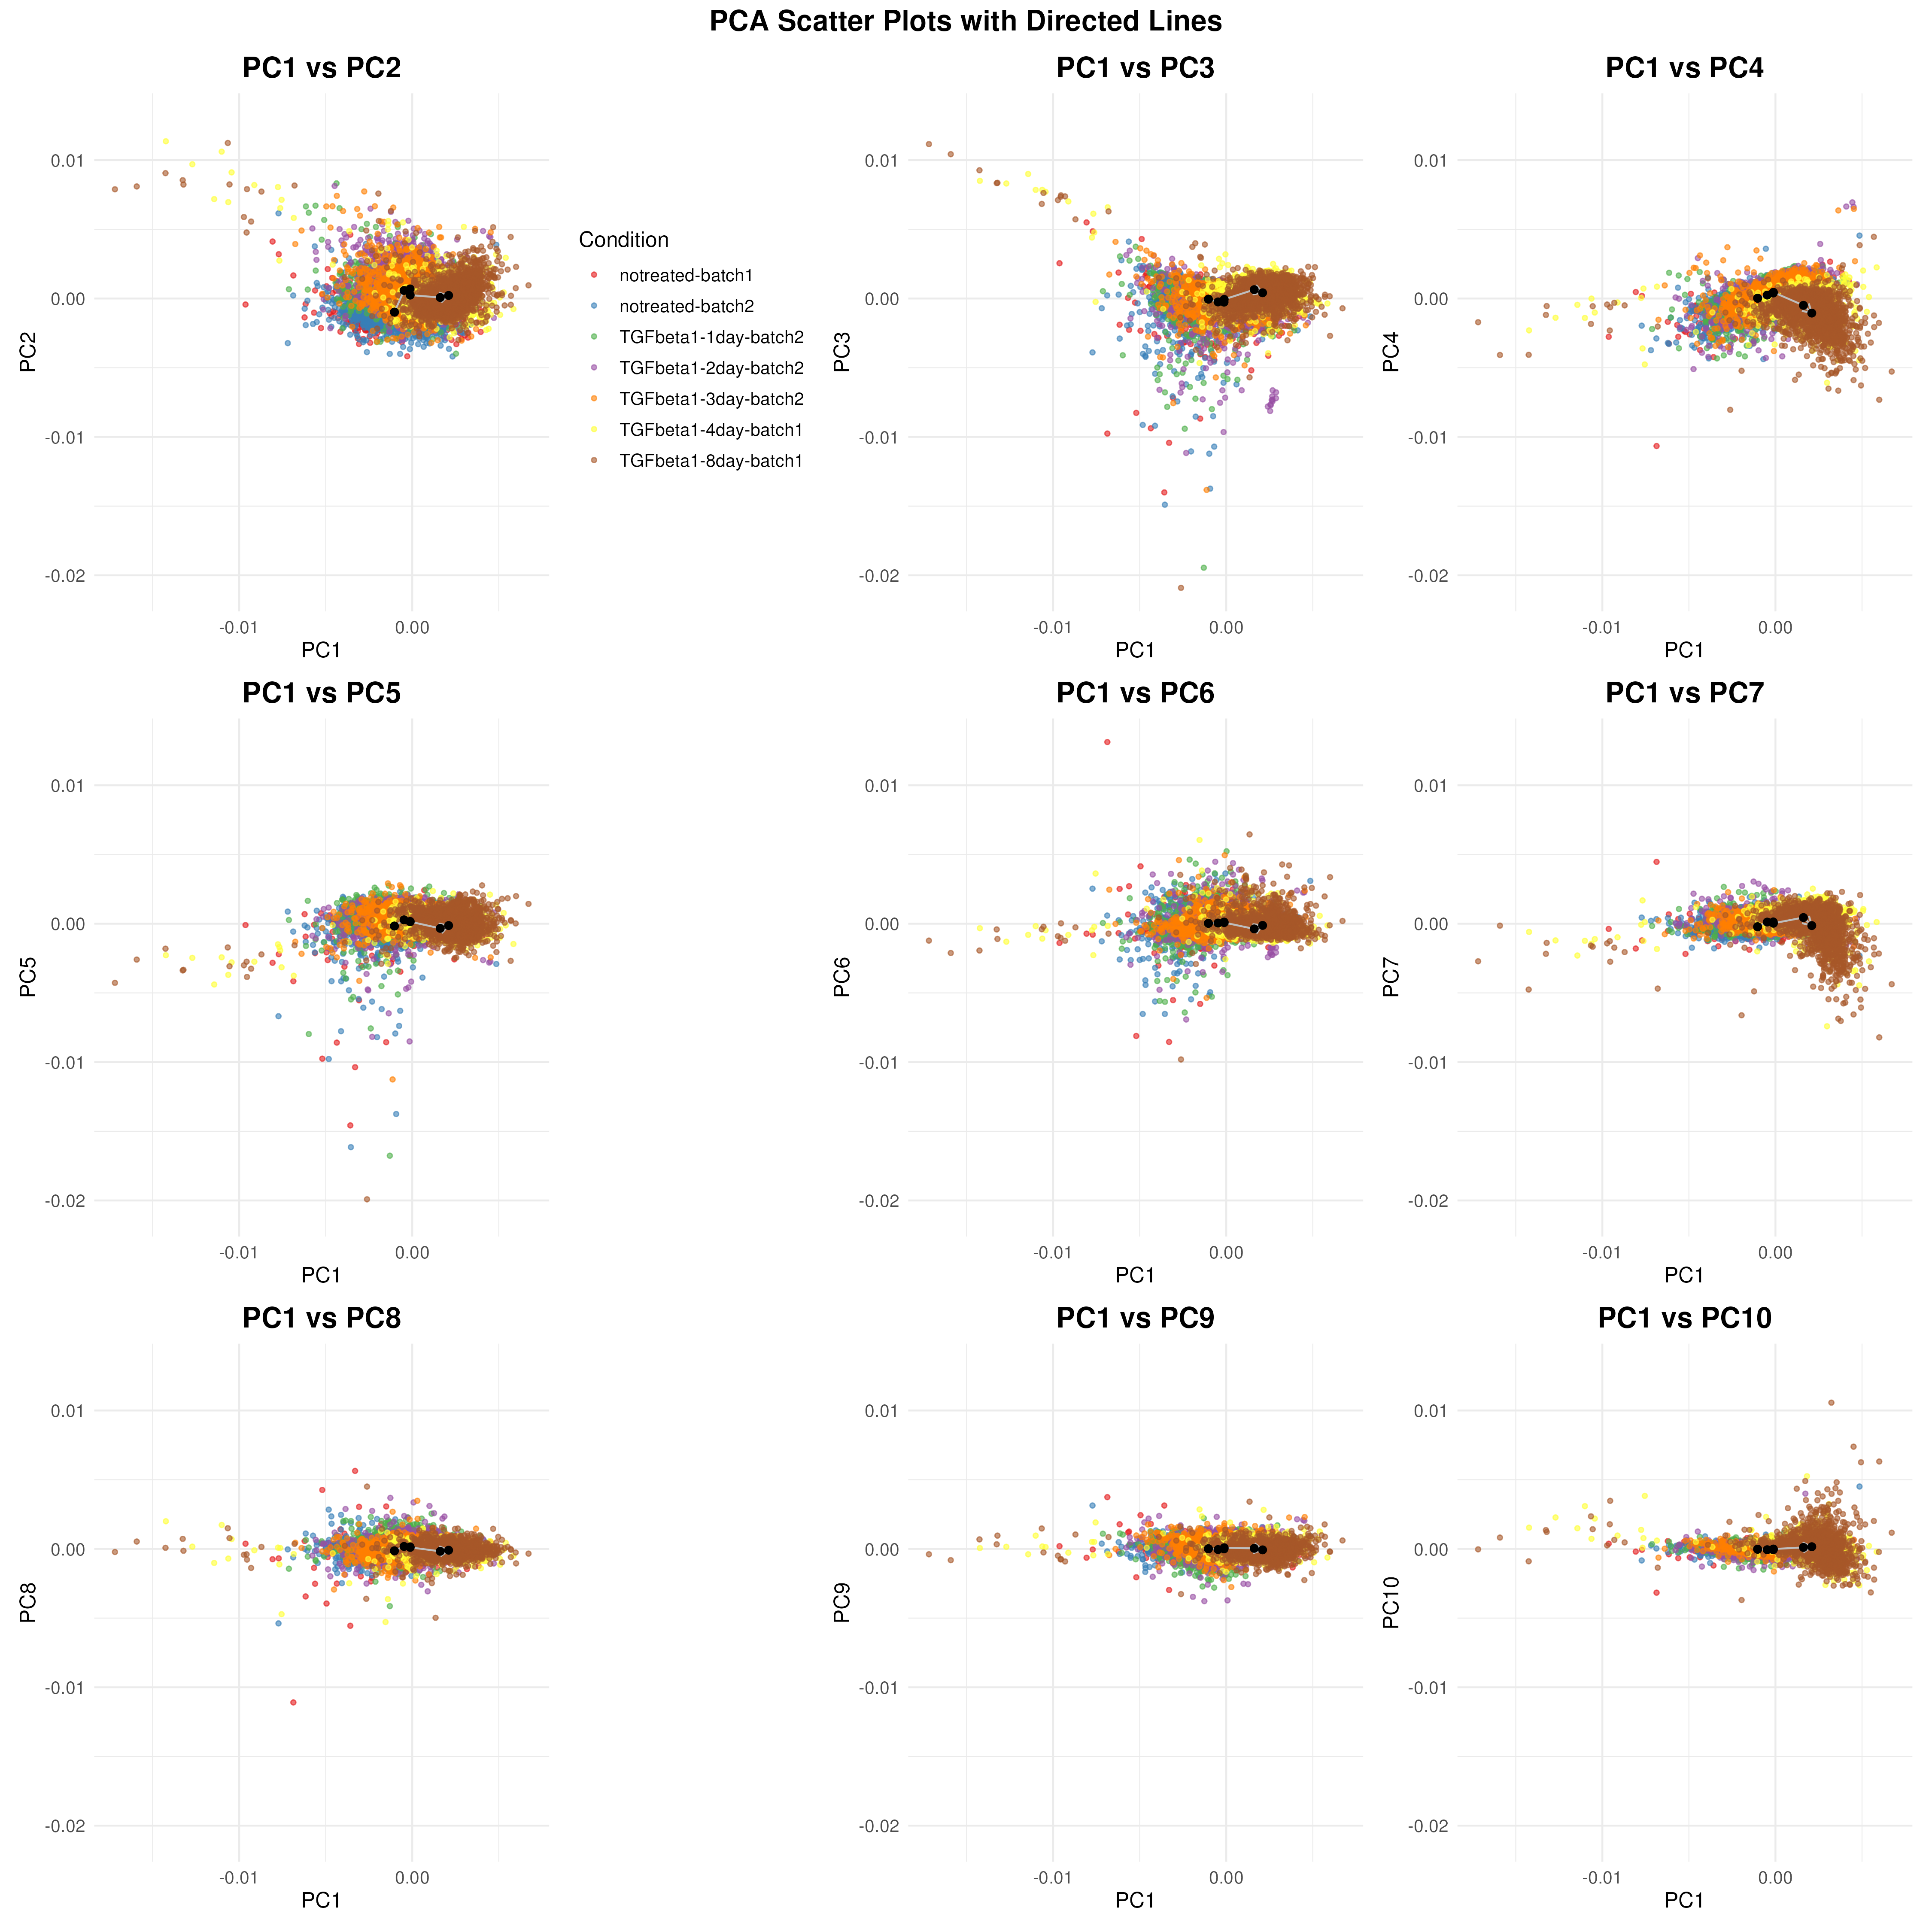
\includegraphics[width=0.75\linewidth]{PCA_Scatter_R0_with_Lines.png}
    \caption{Distribuição PCA Top 10 - R0}
    \label{fig:enter-label}
\end{figure}

\begin{figure}
    \centering
    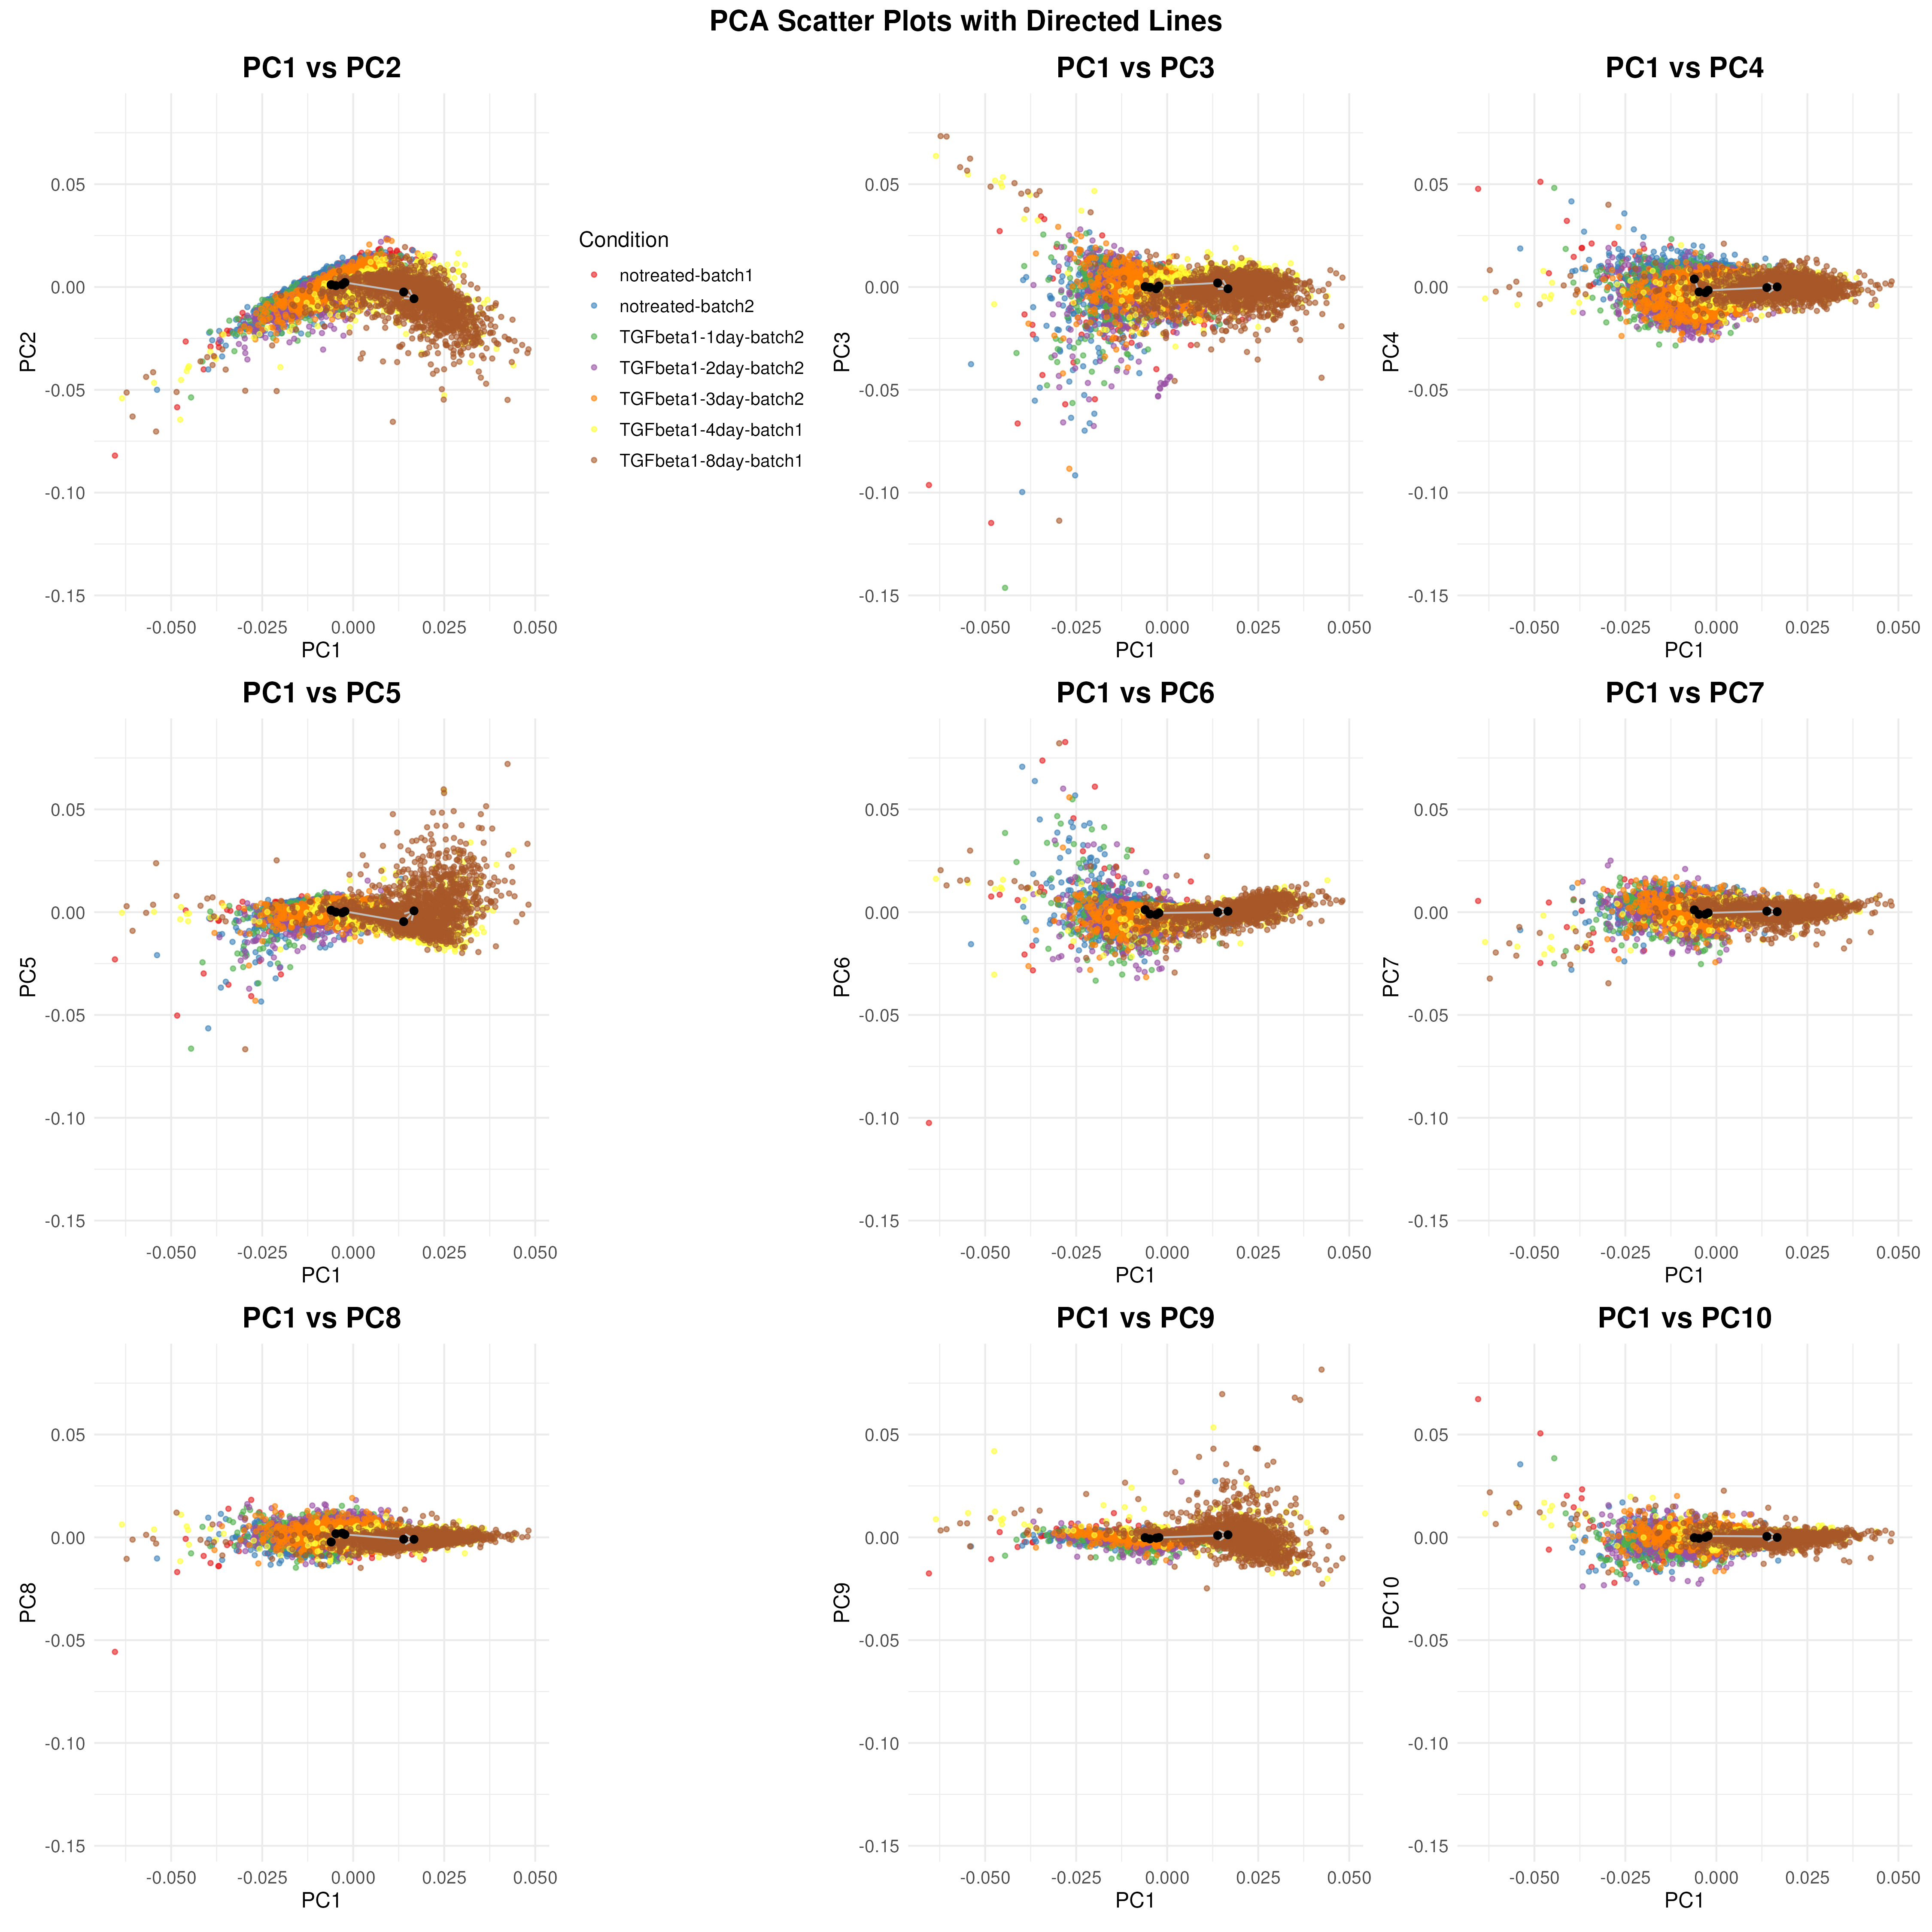
\includegraphics[width=0.75\linewidth]{PCA_Scatter_R30_with_Lines.png}
    \caption{Distribuição PCA Top 10 - R30}
    \label{fig:enter-label}
\end{figure}

\begin{figure}
    \centering
    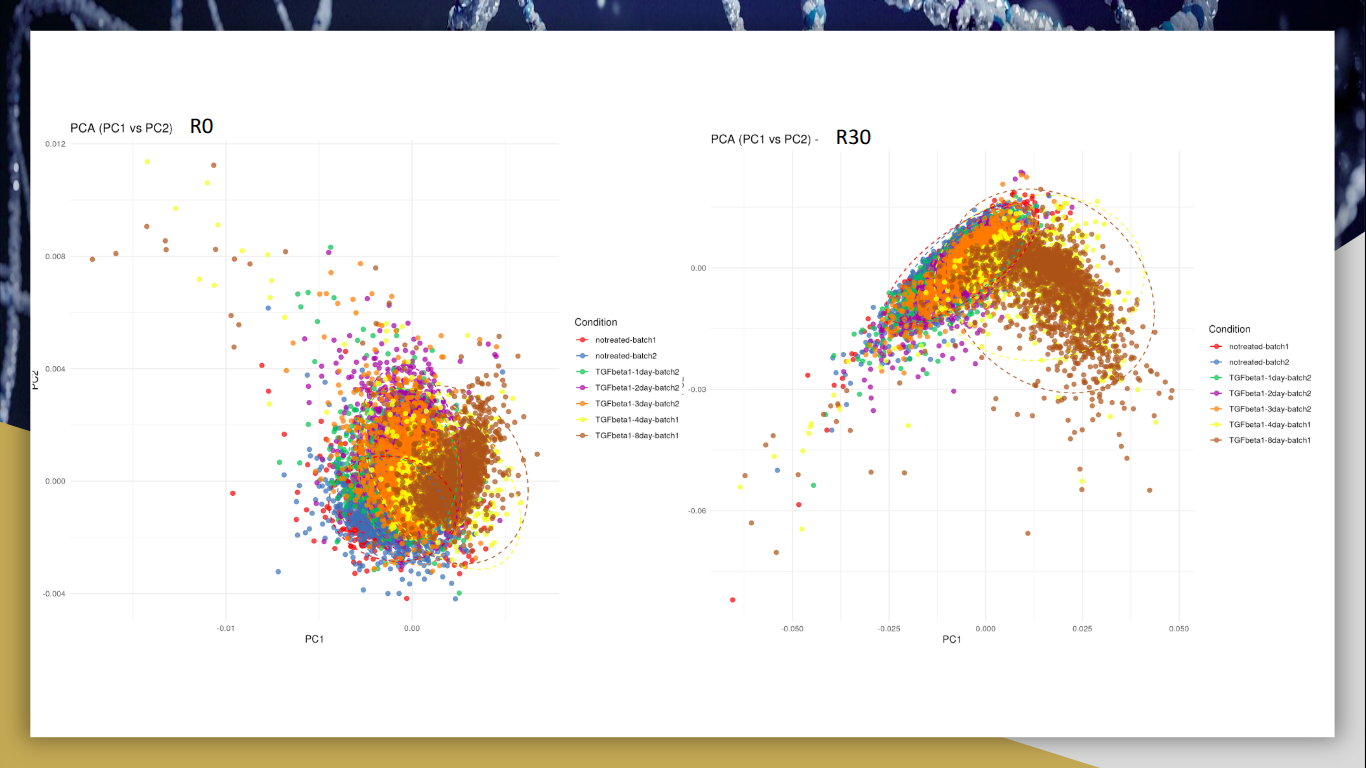
\includegraphics[width=0.75\linewidth]{Captura de tela de 2025-02-11 00-09-09.png}
    \caption{PCA - Comparativo De Agrupamentos R0 e R30 }
    \label{fig:enter-label}
\end{figure}

\begin{figure}
    \centering
    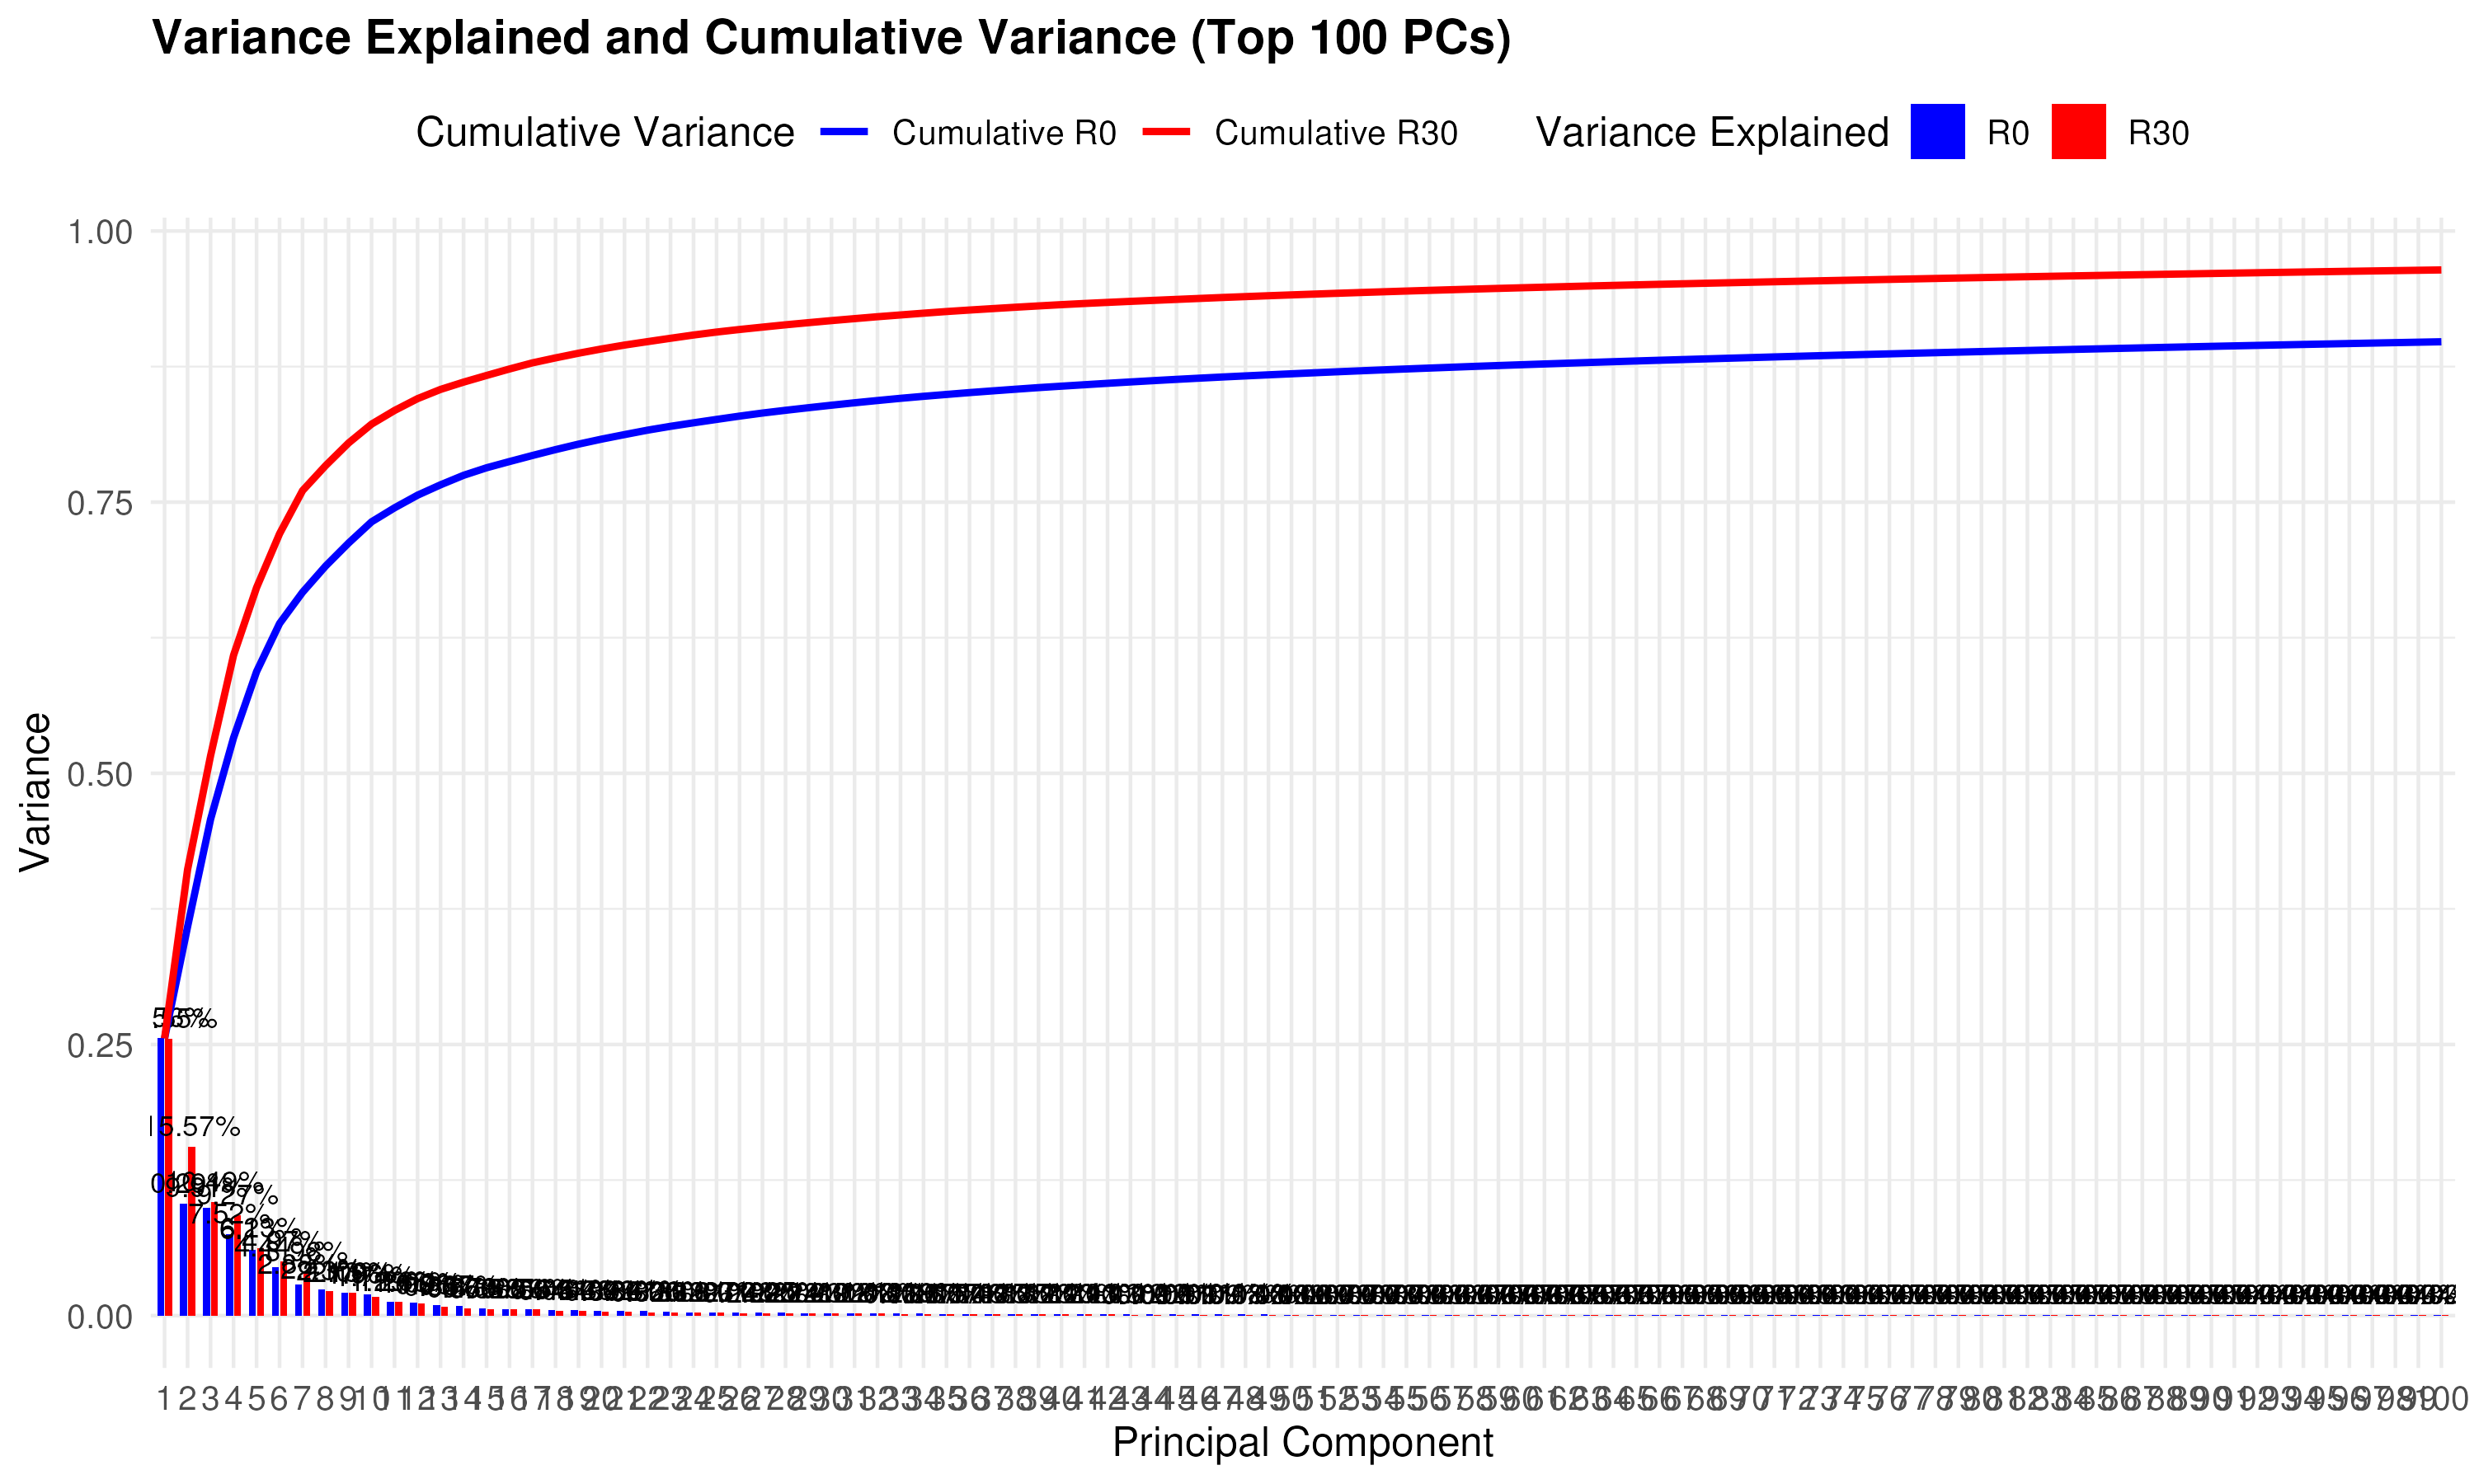
\includegraphics[width=0.75\linewidth]{variance_explained_top100.png}
    \caption{PCA - Comparativo R0 e R30 - Top 10 Componentes Principais}
    \label{fig:enter-label}
\end{figure}

\begin{figure}
    \centering
    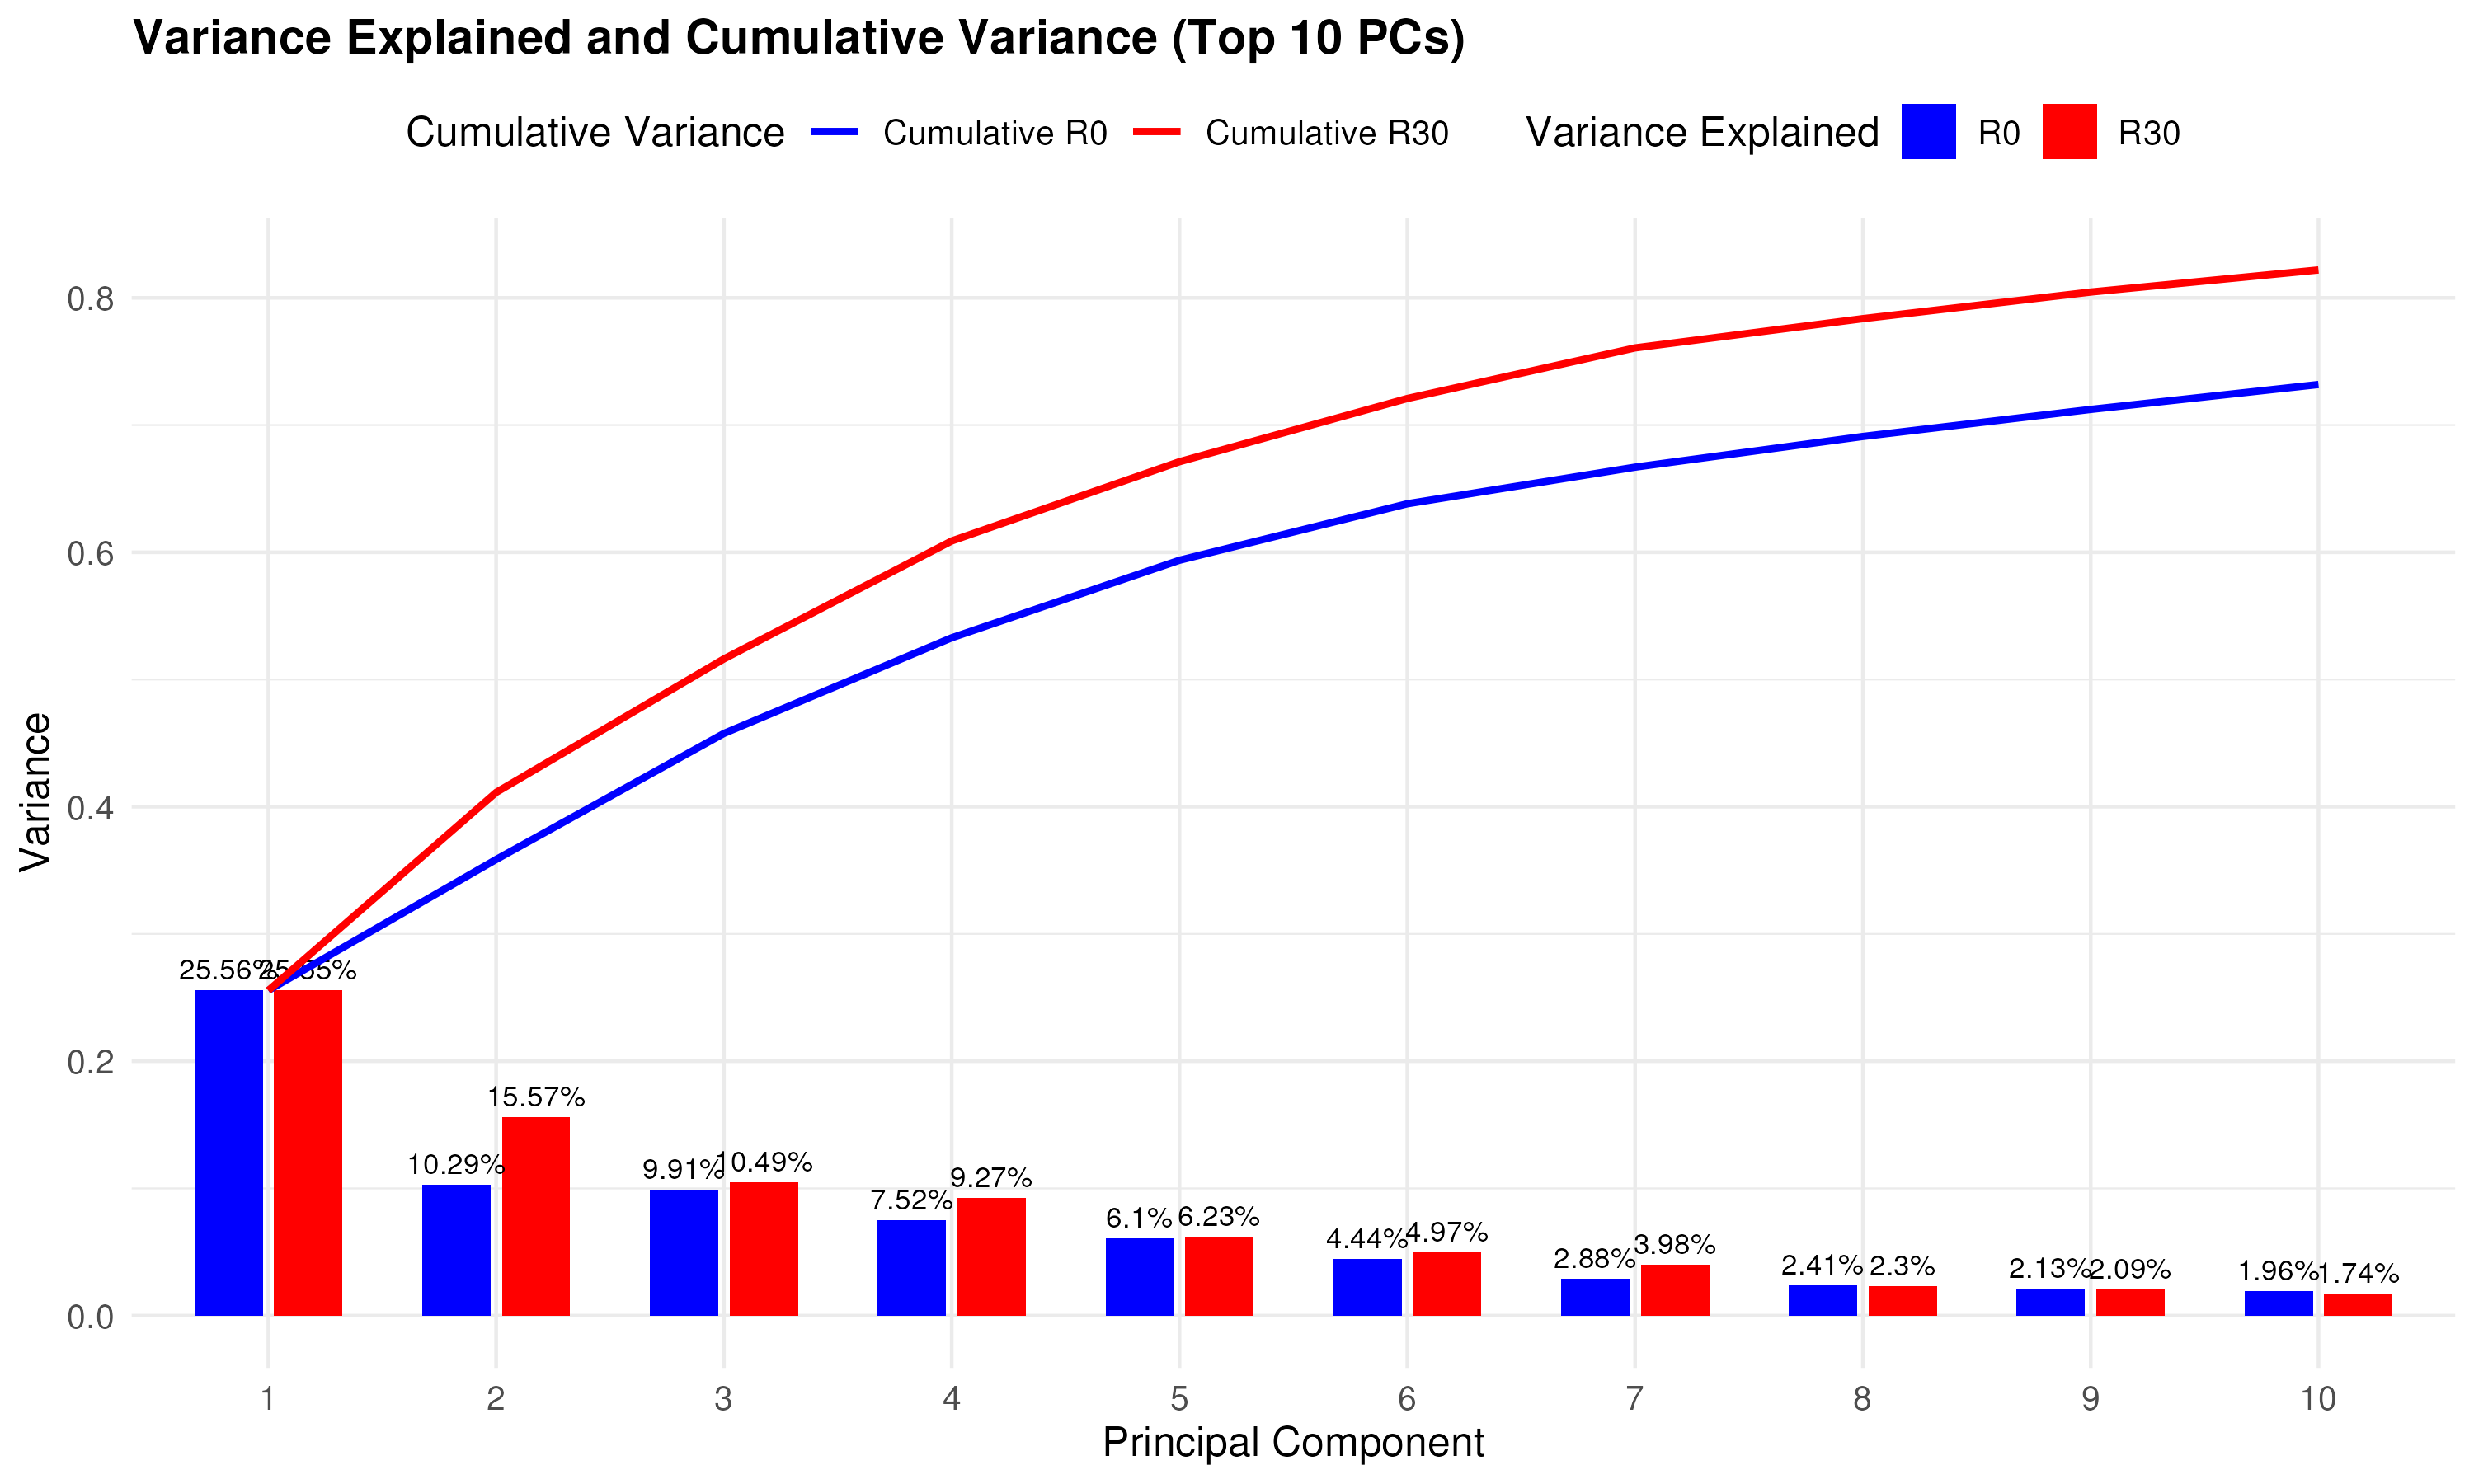
\includegraphics[width=0.75\linewidth]{variance_explained_top10.png}
    \caption{PCA - Comparativo R0 e R30 - Top 10 Componentes Principais}
    \label{fig:enter-label}
\end{figure}

\newpage

\subsection{Distribuição Comparativa dos Coeficientes da PC1}
Nesta seção, analisamos a distribuição comparativa dos coeficientes da primeira componente principal (PC1) considerando todas as proteínas ordenadas conforme uma abordagem biológica. A ordenação das proteínas segue critérios biológicos que possibilitam uma interpretação funcional mais intuitiva da distribuição dos coeficientes da PC1.

\begin{figure}
    \centering
    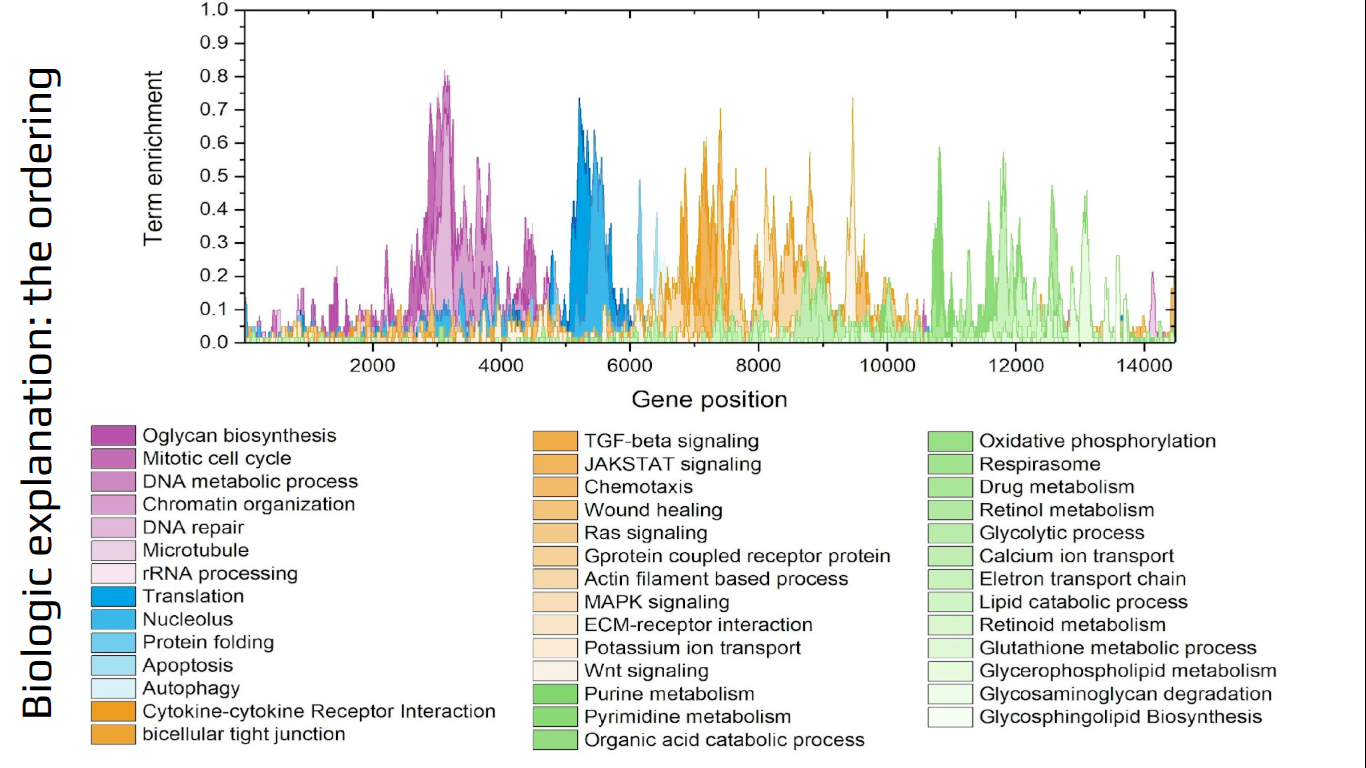
\includegraphics[width=0.75\linewidth]{Captura de tela de 2025-02-11 13-55-24.png}
    \caption{Biologic explanation: the ordering}
    \label{fig:enter-label}
\end{figure}

Para tal, os coeficientes foram extraídos e classificados de acordo com sua posição na sequência biológica estabelecida. A visualização destes coeficientes foi realizada através de gráficos que destacam padrões estruturais e funcionais na distribuição dos valores da PC1. Essa abordagem permite verificar possíveis agrupamentos ou tendências associadas a grupos de proteínas com funções similares.

\begin{figure}
    \centering
    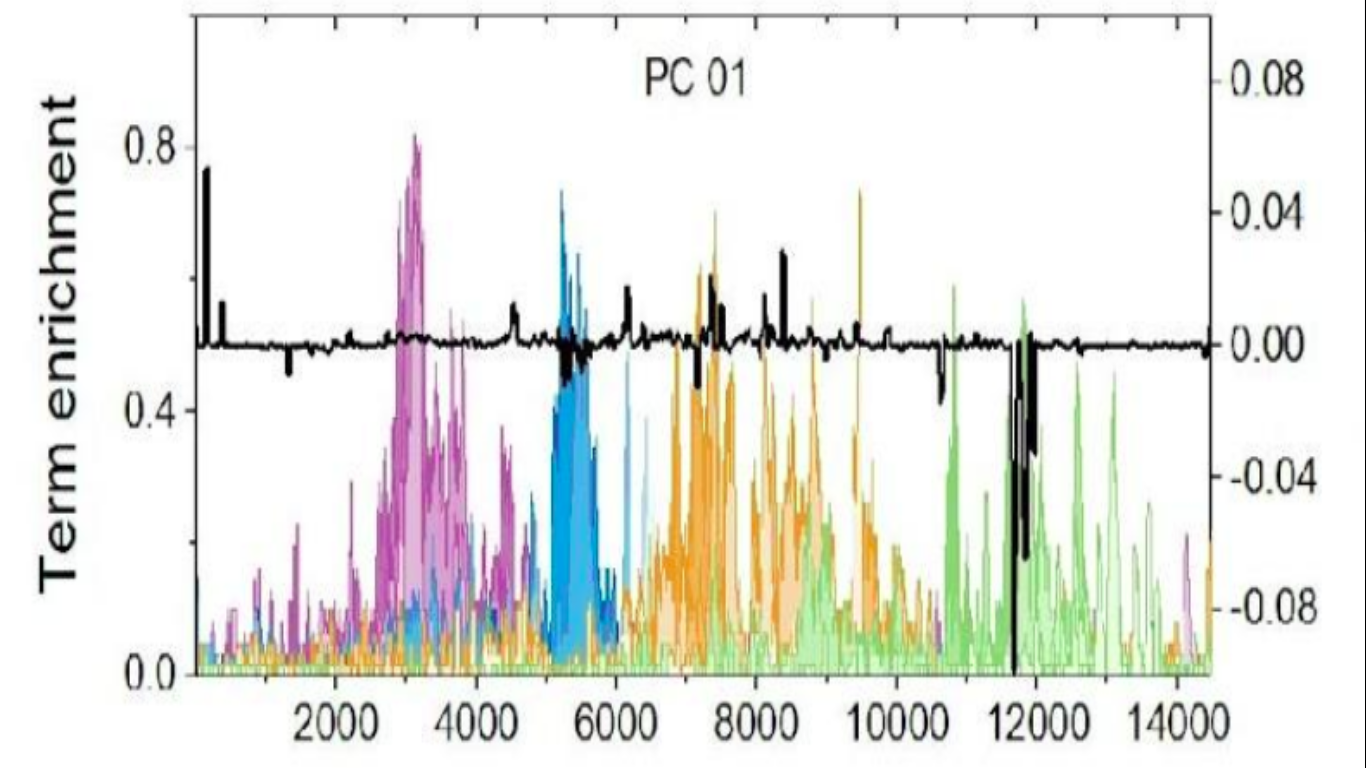
\includegraphics[width=0.75\linewidth]{Biologic explanation: the ordering - Components PC1.png}
    \caption{Biologic explanation: the ordering - Components PC1}
    \label{fig:enter-label}
\end{figure}

Essa análise pode ser expandida para outras componentes principais, possivelmente até as cinco primeiras PCs, a depender dos resultados observados em análises anteriores. A extensão da abordagem permitirá verificar se padrões semelhantes emergem em outras componentes principais, contribuindo para uma compreensão mais aprofundada das principais variações nos dados.

\begin{figure}
    \centering
    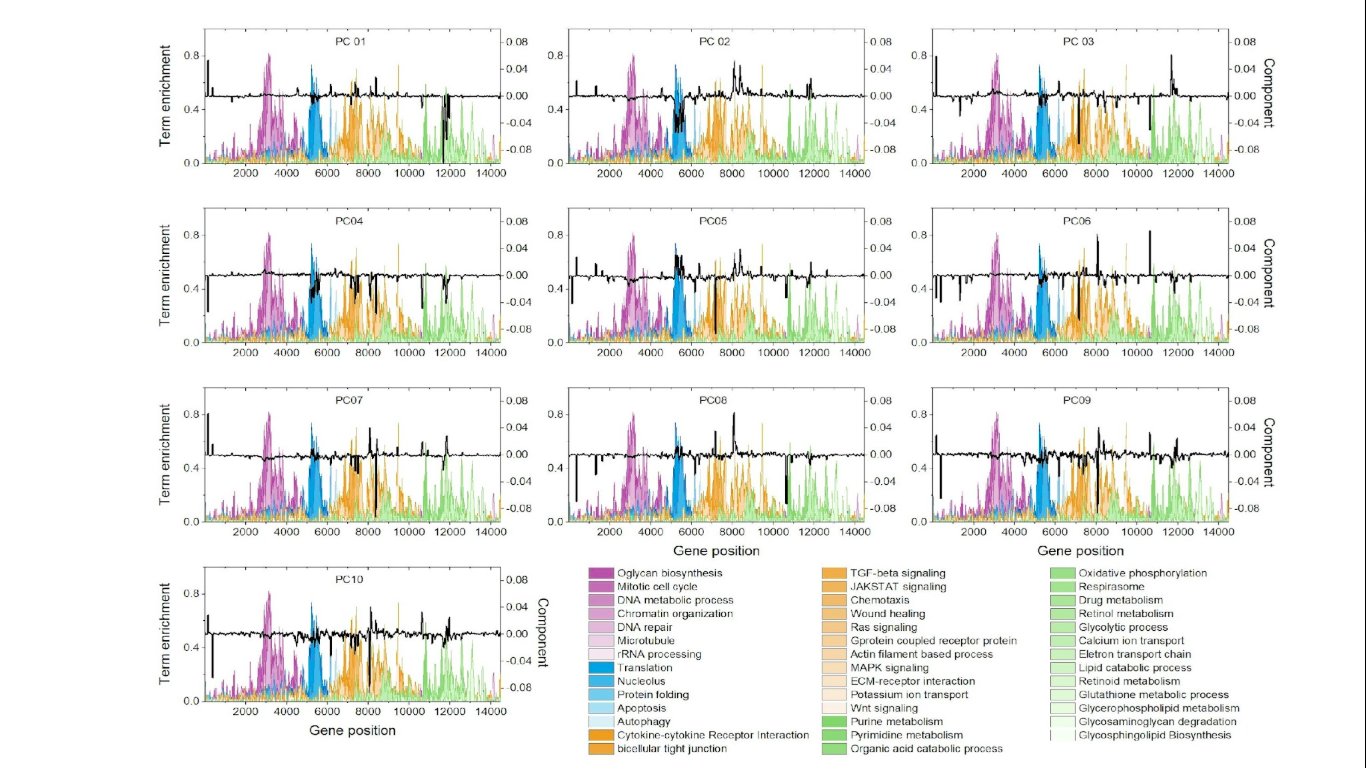
\includegraphics[width=0.75\linewidth]{Biologic explanation: the ordering 10 PCs.png}
    \caption{Biologic explanation: the ordering - Main PCs}
    \label{fig:enter-label}
\end{figure}

\newpage

\subsection{Próximos Passos}
Com base nos resultados obtidos até o momento, os próximos passos envolvem aprofundar a análise da reconstrução do transcriptograma das células a partir das componentes principais. A abordagem seguirá os seguintes pontos:

\begin{itemize}
    \item Reconstrução do transcriptograma da célula $J$ a partir das componentes principais, utilizando a equação:
\begin{equation}
\text{Transcriptograma reconstruído} = \text{rotation} \times \text{t(componentes)} + \text{centro de massa},
\end{equation}
onde o centro de massa corresponde à média de cada linha (gene), resultando em um vetor com o mesmo número de linhas dos genes.

\item Cálculo do coeficiente de determinação ($R^2$) para avaliar a qualidade da reconstrução, definido como:
\begin{equation}
    R^2 = \frac{(\text{amostra}_i - \text{amostra}_i')^2}{\text{quadrado da média do gene}_i},
\end{equation}
onde a média dos valores de $R^2$ será calculada tanto para células quanto para genes.

\item Para cada combinação de componentes principais (por exemplo, utilizando apenas as 3 primeiras PCs), será determinado um valor de $R^2$, representando o erro de reconstrução.

\item Construção de uma curva "Erro x Número de PCs", visando identificar a partir de qual número de componentes a influência se torna irrelevante para a reconstrução.


\begin{equation}
    R^2= \frac{1}{N_{células}N_{genes}} \sum_{j=1}^{N_{células}} \sum_{i=1}^{N_{genes}} \frac{(T_i^{j}-T'_i^{j})^2}{Tmed_i^2},
\end{equation}
onde $T_i^j$ é o valor do transcriptograma da amostra $j$ referente ao gene $i$, $T'_i^j$ é o valor do transcriptograma reconstruido da amostra $j$ referente ao gene $i$ e $Tmed_i$ é o valor médio referente ao gene $i$, tomado sobre todas as células, isto é
\begin{equation}
Tmed_i= \frac{1}{N_{células}} \sum_{j=1}^{N_{células}} T_i^j
\end{equation}

\end{itemize}

Essa análise permitirá compreender melhor a quantidade ideal de componentes principais necessárias para capturar a variação essencial dos dados, otimizando a interpretação e reduzindo a dimensionalidade de forma eficiente.


\newpage

%%%%%% REFERÊNCIAS %%%%%%
\section{Referências}
\begin{thebibliography}{99}
\bibitem[1]{dongre} DONGRE, A.; WEINBERG, R. A. New insights into the mechanisms of epithelial–mesenchymal transition and implications for cancer. \textbf{Nature Reviews Molecular Cell Biology}, v. 20, p. 69–84, 2019.
\bibitem[2]{morais} MORAIS, D. A. A.; ALMEIDA, R. M. C.; DALMOLIN, R. J. S. Transcriptogramer: an R/Bioconductor package for transcriptional analysis based on protein–protein interaction. \textbf{Bioinformatics}, v. 35, n. 16, p. 2875–2876, 2019.
\bibitem[3]{rybarczyk} RYBARCZYK-FILHO, J. L.; CASTRO, M. A.; DALMOLIN, R. J. S.; MOREIRA, J. C.; BRUNNET, L. G.; DE ALMEIDA, R. M. Towards a genome-wide transcriptogram: the \textit{Saccharomyces cerevisiae} case. \textbf{Nucleic Acids Research}, v. 39, n. 8, p. 3005–3016, 2011.
\bibitem[4]{deshmukh} DESHMUKH, A. P.; VASAIKAR, S. V.; TOMCZAK, K.; TRIPATHI, S.; DEN HOLLANDER, P.; ARSLAN, E.; CHAKRABORTY, P.; SOUNDARARAJAN, R.; JOLLY, M. K.; RAI, K.; LEVINE, H.; MANI, S. A. Identification of EMT signaling cross-talk and gene regulatory networks by single-cell RNA sequencing. \textbf{Proceedings of the National Academy of Sciences}, v. 118, n. 19, e2102050118, 2021. DOI: \href{https://doi.org/10.1073/pnas.2102050118}{10.1073/pnas.2102050118}.
\bibitem[5]{deAlmeida2020} DE ALMEIDA, R. M. C.; DE SOUZA, L. L. S.; MORAIS, D.; DALMOLIN, R. J. S. Transcriptograms: A Genome-Wide Gene Expression Analysis Method. In: DA SILVA, F. A. B.; CARELS, N.; TRINDADE DOS SANTOS, M.; LOPES, F. J. P. (eds) \textit{Networks in Systems Biology}. Computational Biology, vol 32. Springer, Cham, 2020. DOI: \href{https://doi.org/10.1007/978-3-030-51862-2_5}{10.1007/978-3-030-51862-2_5}.

\end{thebibliography}




\end{document}
